\documentclass[a4paper,oneside,12pt]{article}
\usepackage[english]{babel}
\usepackage[utf8]{inputenc}
\usepackage[T1]{fontenc}
\usepackage{amsmath,amsthm,amsfonts,amscd,amssymb}
\usepackage{enumitem}
\usepackage{tikz}

\usetikzlibrary{arrows.meta}
\usetikzlibrary{arrows}
\usetikzlibrary{decorations.pathreplacing}

\usepackage[numeric,initials,nobysame,msc-links,abbrev]{amsrefs}
\renewcommand{\eprint}[1]{\href{https://arxiv.org/abs/#1}{arXiv:#1}}
\newcommand{\pageafter}[1]{#1~pp.}
\BibSpec{article}{%
+{} {\PrintAuthors} {author}
+{,} { \textit} {title}
+{.} { } {part}
+{:} { \textit} {subtitle}
+{,} { \PrintContributions} {contribution}
+{.} { \PrintPartials} {partial}
+{,} { } {journal}
+{} { \textbf} {volume}
+{} { \PrintDatePV} {date}
+{,} { \issuetext} {number}
+{,} { \pageafter} {pages}
+{,} { } {status}
+{,} { \PrintDOI} {doi}
+{,} { available at \eprint} {eprint}
+{} { \parenthesize} {language}
+{} { \PrintTranslation} {translation}
+{;} { \PrintReprint} {reprint}
+{.} { } {note}
+{.} {} {transition}
+{} {\SentenceSpace \PrintReviews} {review}
}
\BibSpec{collection.article}{%
+{} {\PrintAuthors} {author}
+{,} { \textit} {title}
+{.} { } {part}
+{:} { \textit} {subtitle}
+{,} { \PrintContributions} {contribution}
+{,} { \PrintConference} {conference}
+{} {\PrintBook} {book}
+{,} { } {booktitle}
+{,} { \PrintDateB} {date}
+{,} { \pageafter} {pages}
+{,} { } {status}
+{,} { \PrintDOI} {doi}
+{,} { available at \eprint} {eprint}
+{} { \parenthesize} {language}
+{} { \PrintTranslation} {translation}
+{;} { \PrintReprint} {reprint}
+{.} { } {note}
+{.} {} {transition}
+{} {\SentenceSpace \PrintReviews} {review}
}
\usepackage{longtable,geometry}
\usepackage{graphicx}
\usepackage{authblk}
\usepackage{pstricks}
\usepackage{bbm}
\usepackage{hyperref}
\usepackage[capitalise]{cleveref}
\usepackage{xparse}
%\usepackage[notref,notcite]{showkeys}

\geometry{dvips,a4paper,margin=1.5in}


\setlist[itemize]{leftmargin=*}
\setlist[enumerate]{leftmargin=*,label=(\arabic*),ref=(\arabic*)}

\setlength{\topmargin}{-1.5cm}
\setlength{\headsep}{0.3cm}
\setlength{\textheight}{22.5cm}
\setlength{\oddsidemargin}{0.5cm}
\setlength{\evensidemargin}{0.5cm}
\setlength{\textwidth}{16.0cm}
%% resetting nasty Latex defaults
\tolerance 500

\newtheorem{theorem}{Theorem}
\crefname{theorem}{Theorem}{Theorems}
\newtheorem{corollary}[theorem]{Corollary}
\crefname{corollary}{Corollary}{Corollaries}
\newtheorem{lemma}[theorem]{Lemma}
\crefname{lemma}{Lemma}{Lemmas}
\newtheorem{proposition}[theorem]{Proposition}
\crefname{proposition}{Proposition}{Propositions}
\newtheorem{conjecture}[theorem]{Conjecture}
\crefname{conjecture}{Conjecture}{Conjectures}
\newtheorem{question}{Question}
\crefname{question}{Question}{Questions}
\theoremstyle{definition}
\newtheorem{definition}[theorem]{Definition}
\crefname{definition}{Definition}{Definitions}
\newtheorem{remark}[theorem]{Remark}
\crefname{remark}{Remark}{Remarks}
\newtheorem{example}[theorem]{Example}
\crefname{example}{Example}{Examples}
\newtheorem{observation}[theorem]{Observation}
\crefname{observation}{Observation}{Observations}
\newtheorem{claim}[theorem]{Claim}
\crefname{claim}{Claim}{Claims}
\newtheorem{assumption}[theorem]{Assumption}
\crefname{assumption}{Assumption}{Assumptions}

\numberwithin{theorem}{section}
\numberwithin{equation}{section}

\newcommand{\Z}{\mathbb{Z}}
\newcommand{\N}{\mathbb{N}}
\newcommand{\R}{\mathbb{R}}
\renewcommand{\P}{\mathbb{P}}
\newcommand{\F}{\mathcal{F}}
\newcommand{\G}{\mathcal{G}}
\renewcommand{\L}{\mathcal{L}}
\newcommand{\Rplus}{\mathbb{R}_+}
\newcommand{\Qplus}{\mathbb{Q}_+}
\newcommand{\C}{\mathbb{C}}
\renewcommand{\H}{\mathbb{H}}
\newcommand{\Hbar}{\overline{\mathbb{H}}}
\newcommand{\Half}{\mathbb{H}}
\newcommand{\Disk}{\mathbb{D}}
\newcommand{\B}{\mathcal{B}}
\renewcommand{\S}{\mathcal{S}}
\newcommand{\T}{\mathcal{T}}
\newcommand{\NN}{\mathcal{N}}
\newcommand{\U}{\mathbb{U}}
\newcommand{\g}{\gamma}
\newcommand{\D}{\mathcal{D}}
\newcommand{\I}{\mathcal{I}}
\newcommand{\A}{\mathcal{A}}
\newcommand{\E}{\mathcal{E}}
\newcommand{\e}{\varepsilon}
\newcommand{\HH}{\mathcal{H}}

%%%%%%%%%%%%%%%%%%%%%%%%%%%%%%%%%%%%%%%%%%%%%%%%%%%%%%%%%%%%%%%%%%%%%%%%%%%%%%
%%%%%%%%%% Calligraphic letters
%%%%%%%%%%%%%%%%%%%%%%%%%%%%%%%%%%%%%%%%%%%%%%%%%%%%%%%%%%%%%%%%%%%%%%%%%%%%%%
\newcommand{\cA}{\ensuremath{\mathcal A}}
\newcommand{\cB}{\ensuremath{\mathcal B}}
\newcommand{\cC}{\ensuremath{\mathcal C}}
\newcommand{\cD}{\ensuremath{\mathcal D}}
\newcommand{\cE}{\ensuremath{\mathcal E}}
\newcommand{\cF}{\ensuremath{\mathcal F}}
\newcommand{\cG}{\ensuremath{\mathcal G}}
\newcommand{\cH}{\ensuremath{\mathcal H}}
\newcommand{\cI}{\ensuremath{\mathcal I}}
\newcommand{\cJ}{\ensuremath{\mathcal J}}
\newcommand{\cK}{\ensuremath{\mathcal K}}
\newcommand{\cL}{\ensuremath{\mathcal L}}
\newcommand{\cM}{\ensuremath{\mathcal M}}
\newcommand{\cN}{\ensuremath{\mathcal N}}
\newcommand{\cO}{\ensuremath{\mathcal O}}
\newcommand{\cP}{\ensuremath{\mathcal P}}
\newcommand{\cQ}{\ensuremath{\mathcal Q}}
\newcommand{\cR}{\ensuremath{\mathcal R}}
\newcommand{\cS}{\ensuremath{\mathcal S}}
\newcommand{\cT}{\ensuremath{\mathcal T}}
\newcommand{\cU}{\ensuremath{\mathcal U}}
\newcommand{\cV}{\ensuremath{\mathcal V}}
\newcommand{\cW}{\ensuremath{\mathcal W}}
\newcommand{\cX}{\ensuremath{\mathcal X}}
\newcommand{\cY}{\ensuremath{\mathcal Y}}
\newcommand{\cZ}{\ensuremath{\mathcal Z}}

%%%%%%%%%%%%%%%%%%%%%%%%%%%%%%%%%%%%%%%%%%%%%%%%%%%%%%%%%%%%%%%%%%%%%%%%%%%%%%
%%%%%%%%%%%% Blackboard bolds
%%%%%%%%%%%%%%%%%%%%%%%%%%%%%%%%%%%%%%%%%%%%%%%%%%%%%%%%%%%%%%%%%%%%%%%%%%%%%%

\newcommand{\bbA}{{\ensuremath{\mathbb A}} }
\newcommand{\bbB}{{\ensuremath{\mathbb B}} }
\newcommand{\bbC}{{\ensuremath{\mathbb C}} }
\newcommand{\bbD}{{\ensuremath{\mathbb D}} }
\newcommand{\bbE}{{\ensuremath{\mathbb E}} }
\newcommand{\bbF}{{\ensuremath{\mathbb F}} }
\newcommand{\bbG}{{\ensuremath{\mathbb G}} }
\newcommand{\bbH}{{\ensuremath{\mathbb H}} }
\newcommand{\bbI}{{\ensuremath{\mathbb I}} }
\newcommand{\bbJ}{{\ensuremath{\mathbb J}} }
\newcommand{\bbK}{{\ensuremath{\mathbb K}} }
\newcommand{\bbL}{{\ensuremath{\mathbb L}} }
\newcommand{\bbM}{{\ensuremath{\mathbb M}} }
\newcommand{\bbN}{{\ensuremath{\mathbb N}} }
\newcommand{\bbO}{{\ensuremath{\mathbb O}} }
\newcommand{\bbP}{{\ensuremath{\mathbb P}} }
\newcommand{\bbQ}{{\ensuremath{\mathbb Q}} }
\newcommand{\bbR}{{\ensuremath{\mathbb R}} }
\newcommand{\bbS}{{\ensuremath{\mathbb S}} }
\newcommand{\bbT}{{\ensuremath{\mathbb T}} }
\newcommand{\bbU}{{\ensuremath{\mathbb U}} }
\newcommand{\bbV}{{\ensuremath{\mathbb V}} }
\newcommand{\bbW}{{\ensuremath{\mathbb W}} }
\newcommand{\bbX}{{\ensuremath{\mathbb X}} }
\newcommand{\bbY}{{\ensuremath{\mathbb Y}} }
\newcommand{\bbZ}{{\ensuremath{\mathbb Z}} }


\newcommand{\ba}{\ensuremath{\mathbf{a} }}
\newcommand{\bb}{\ensuremath{\mathbf{b} }}
\newcommand{\bc}{\ensuremath{\mathbf{c} }}
\newcommand{\bd}{\ensuremath{\mathbf{d} }}
\newcommand{\be}{\ensuremath{\mathbf{e} }}
%\newcommand{\bf}{\ensuremath{\mathbf{f} }}
\newcommand{\bg}{\ensuremath{\mathbf{g} }}
\newcommand{\bh}{\ensuremath{\mathbf{h} }}
\newcommand{\bi}{\ensuremath{\mathbf{i} }}
\newcommand{\bj}{\ensuremath{\mathbf{j} }}
\newcommand{\bk}{\ensuremath{\mathbf{k} }}
\newcommand{\bl}{\ensuremath{\mathbf{l} }}
\newcommand{\bm}{\ensuremath{\mathbf{m} }}
\newcommand{\bn}{\ensuremath{\mathbf{n} }}
\newcommand{\bo}{\ensuremath{\mathbf{o} }}
\newcommand{\bp}{\ensuremath{\mathbf{p} }}
\newcommand{\bq}{\ensuremath{\mathbf{q} }}
\newcommand{\br}{\ensuremath{\mathbf{r} }}
\newcommand{\bs}{\ensuremath{\mathbf{s} }}
\newcommand{\bt}{\ensuremath{\mathbf{t} }}
\newcommand{\bu}{\ensuremath{\mathbf{u} }}
\newcommand{\bv}{\ensuremath{\mathbf{v} }}
\newcommand{\bw}{\ensuremath{\mathbf{w} }}
\newcommand{\bx}{\ensuremath{\mathbf{x} }}
\newcommand{\by}{\ensuremath{\mathbf{y} }}
\newcommand{\bz}{\ensuremath{\mathbf{z} }}


\newcommand{\<}{\langle}
\renewcommand{\>}{\rangle}

\newcommand{\1}{{\ensuremath{\mathbbm{1}}} }

\DeclareDocumentCommand \to { o o } {%
  \IfNoValueTF {#1} {\IfNoValueTF{#2}{\rightarrow}{\xrightarrow[#2]}}%
{\IfNoValueTF{#2}{\xrightarrow{#1}}{\xrightarrow[#2]{#1}}}}
\DeclareDocumentCommand \nto { o } {%
  \IfNoValueTF {#1} {{\ensuremath{\centernot{\rightarrow}}} }{{\ensuremath{\centernot{\xrightarrow{#1}}}}}%
}

\DeclareMathOperator{\diam}{diam}
\DeclareMathOperator{\Pod}{Pod}

\newcommand{\ih}[1]{{\color{red}{#1}}}
\newcommand{\ivh}[1]{{\color{orange}{#1}}}
\newcommand{\hd}[1]{{\color{blue}{#1}}}
\newcommand{\hdc}[1]{{\color{magenta}{#1}}}
 
%%%%%%%%%%%%%%%%%%%%%%
%title, authors and date
%%%%%%%%%%%%%%%%%%%%%%

\title{Sharp metastability transition for two-dimensional bootstrap percolation with symmetric isotropic threshold rules}
\date{\today}
\author[1,2]{Hugo Duminil-Copin}
\author[3]{Ivailo Hartarsky}
\affil[1]{University of Geneva}
\affil[2]{Institut des Hautes \'Etudes Scientifiques}
\affil[3]{TU Wien, Faculty of Mathematics and Geoinformation, Institute of Statistics and Mathematical Methods in Economics, Research Unit of Mathematical Stochastics, Wiedner Hauptstra\ss e 8-10, A-1040 Vienna, Austria, \texttt{ivailo.hartarsky@tuwien.ac.at}}
%%%%%%%%%%%%%%%%%%%%%%%%%%%%%%%%
%beginning of the document
%%%%%%%%%%%%%%%%%%%%%%%%%%%%%%%%
\begin{document}

\maketitle


\begin{abstract} 
We study two-dimensional critical bootstrap percolation models. We establish that a class of these models including all isotropic threshold rules with a convex symmetric neighbourhood, undergoes a sharp metastability transition. This extends previous instances proved for several specific rules. The paper supersedes a draft by Alexander Holroyd and the first author from 2012. While it served a role in the subsequent development of bootstrap percolation universality, we have chosen to adopt a more contemporary viewpoint in its present form.
\end{abstract}

\noindent\textbf{MSC2020:} 60K35; 60C05
\\
\textbf{Keywords:} bootstrap percolation, sharp threshold, metastability

\section{Introduction}
A threshold bootstrap percolation model is a simple cellular automaton that provides a useful model for studying several phenomena such as metastability, dynamics of glasses or crack formation. A famous example of a threshold model is the \emph{$2$-neighbour bootstrap percolation} originally introduced by Chalupa, Leath and Reich \cite{Chalupa79} (also see \cite{Kogut81}). In this model, sites of the square lattice $\mathbb Z^2$ are infected or healthy. At time 0, sites are infected with probability $p$ independently of each other (we denote the corresponding measure by $\mathbb P_p$). At each time step, a site becomes infected if two or more of its nearest neighbours are infected.

The first rigorous result on this model \cite{vanEnter87}, dating back to 1987, established that every site of $\mathbb Z^2$ becomes infected almost surely whenever $p>0$. This motivates the study of the (random) first time $\tau$ at which 0 becomes infected as $p$ goes to 0. In \cite{Aizenman88}, Aizenman and Lebowitz proved that there exist two constants $c,C\in(0,\infty)$ such that
\[\lim_{p\rightarrow 0}\mathbb P_p\left(e^{c/p}\le \tau\le e^{C/p}\right)=1.\] 
We refer to this article for an enlightening exposition of the metastability effects in the model. The question of whether $c$ and $C$ could be chosen arbitrary close to each other was left open for a long time. Finally, a sharp metastability transition was shown to occur in \cite{Holroyd03}: $p\log \tau$ converges in probability to $\pi^2/18$ as  $p\rightarrow 0$. More precise estimates for $T$ were derived later in \cite{Hartarsky19}.

Several authors investigated more general growth rules and the right order of magnitude for $\tau$ is now known for all rules \cite{Bollobas23}, hence generalising the result of Aizenman and Lebowitz. The sharp metastability transition, though, remained available only for a handful of isolated examples \cites{Bollobas17,Duminil-Copin13,Holroyd03,Holroyd03a}. The goal of this paper is to prove sharp metastability for a wide class of models. In particular, we show that every isotropic symmetric convex threshold bootstrap percolation model exhibits a sharp transition.

\subsection{$\cU$-bootstrap percolation}

Let $\Z^2=\{x=(x_1,x_2):x_1,x_2\in \Z\}$ be the set of all 2-vectors of integers and $\mathbb N=\{0,1,\dots\}$. Elements of $\Z^2$ are called {\em sites}. An \emph{update rule} is any finite non-empty subset of $\bbZ^2\setminus\{0\}$. An \emph{update family} is a finite non-empty set of update rules. An update family $\cU$ is \emph{symmetric}, if for every $U\in\cU$ we have $-U=\{-x:x\in U\}\in\cU$. Given an update family $\cU$ and a set $A=A_0\subseteq\bbZ^2$ of \emph{initial infections}, we recursively define
\[A_{t+1}=A_t\cup\{x\in\bbZ^2:\exists U\in\cU,\forall u\in U,x+u\in A_t\}\]
to be the set of sites \emph{infected at time $t$} in the $\cU$-bootstrap percolation process. The set $[A]=\bigcup_{t\ge 0}A_t$ of eventually infected sites is called the \emph{closure} of $A$. A set $A\subseteq\bbZ^2$ is called \emph{stable} if $[A]=A$. An observable of particular interest is the infection time of the origin \[\tau=\inf\{t\in\bbN:0\in A_t\}\in\bbN\cup\{\infty\}.\] We will systematically be interested in the asymptotics of $\tau$ when each site is initially infected independently with probability $p\to 0$. We denote the corresponding distribution of $A$ by $\bbP_p$.

Among all update families, threshold rules initially received particular attention \cite{Gravner99}. They are defined by a finite \emph{neighbourhood} $\cK\subset \bbZ^2$, containing $0$, and a positive integer \emph{threshold} $\theta$. Then \[\cU(\cK,\theta)=\{U\subseteq \cK:|U|=\theta\}\] is the associated update family. In other words, a site $x$ becomes infected if at least $\theta$ of the sites in its neighbourhood $x+\cK$ are already infected. A set $\cK\subseteq \bbR^2$ is called \emph{symmetric} if $x\in \cK$ implies $-x\in \cK$ for all $x\in\bbR^2$. We say that a neighbourhood $\cK\subset \bbZ^2$ is \emph{convex symmetric}, if it is the intersection of a bounded convex symmetric subset of $\bbR^2$ with $\bbZ^2$.

We will require a few definitions from the bootstrap percolation universality framework \cites{Bollobas15,Bollobas23,Gravner99,Hartarsky22univlower}. A \emph{direction} is a unit vector of $\bbR^2$, viewed as an element of the unit circle $S^1$. We denote the open half plane with outer normal $u$ by $\bbH_u=\{x\in\bbZ^2:\<u,x\><0\}$ and its boundary by  $l_u=\{x\in\bbZ^2:\<u,x\>=0\}$. A direction $u\in S^1$ is called \emph{stable}, if $\bbH_u$ is stable. The direction is \emph{unstable} otherwise, which can be reinterpreted as follows: there exists an update rule $U\subset\bbH_u$. In the case of a threshold rule, unstable directions $u$ are those for which $|\bbH_u\cap \cK|\ge \theta$.

A direction $u\in S^1$ is called \emph{rational} if $\lambda u\in \bbZ^2\setminus\{0\}$ for some $\lambda\in\bbR$. In this case, we denote $\rho_u=\min\{\rho>0:\exists x\in\bbZ^2,\<u,x\>=\rho\}$. Then $u\bbR\cap\bbZ^2=(u/\rho_u)\bbZ$. Thus, it will be convenient to define $u^\perp=(u_2,-u_1)/\rho_u$, so that $l_u=u^\perp\bbZ$. We further denote by  $l_u(n)=\{x\in\bbZ^2:\<u,x\>=n\rho_u\}$ the $n$-th line perpendicular to $u$, so that $\bbZ^2=\bigsqcup_{n\in\bbZ}l_u(n)$. Note that for any $n\in\bbZ$, $l_u(n)$ is a translate of $l_u$.

In the present work we will only consider models with finitely many stable directions. For an isolated stable or an unstable direction $u\in S^1$, we define its \emph{difficulty}
\begin{equation}
\label{eq:def:alpha}
\alpha(u)=\min\{|Z|:Z\subset\bbZ^2,|[\bbH_u\cup Z]\setminus\bbH_u|=\infty\}\in\bbN.
\end{equation}
That is, the difficulty of $u$ is the minimal number of infected sites needed in addition to the half-plane $\bbH_u$, so that infinitely many additional sites become infected. An update family is called \emph{isotropic} if it has a finite but nonzero number of stable directions and each open semicircle of $S^1$ contains a stable direction of maximal difficulty. For isotropic models we call \[\alpha=\max_{u\in S^1}\alpha(u)\] the \emph{difficulty} of the update family. A set $Z$ realising the minimum in \cref{eq:def:alpha} is called a \emph{helping set}. A helping set $Z\subset \bbZ^2$ for $u$ is \emph{voracious} if $[\bbH_u\cup Z]\supseteq l_u$. The update family is called \emph{voracious} if all helping sets for all directions of difficulty $\alpha$ are voracious.

It was shown in \cite{Bollobas23} that for every isotropic update family, there exists $C>c>0$ such that 
\[\lim_{p\rightarrow 0}\mathbb P_p\left(e^{ c/p^{\alpha}}<\tau<e^{ C/p^{\alpha}}\right)=1.\]  
One can check that symmetric threshold models are isotropic if and only if the maximum $\iota(\cK)=\max_{u\in S^1}|l_u\cap \cK|$ is attained for at least two non-opposite directions $u$ and $|\cK|-\iota(\cK)<2\theta<|\cK|$. In that case, the difficulty is given by $\alpha=\theta-(|\cK|-\iota(\cK))/2$ and the difficulty of a direction $u\in S^1$ is $\alpha(u)=\max(0,\theta-|\cK\setminus l_u|/2)$ (see \cite{Gravner99}).

\subsection{Main results}
Our main result is the following.
\begin{theorem}\label{th:main}
For any symmetric voracious isotropic update family with difficulty $\alpha$, there exists $\lambda\in(0,\infty)$ such that for all $\varepsilon>0$,
\[\lim_{p\rightarrow0}\mathbb P_p\left(|p^\alpha\log \tau-\lambda|>\varepsilon\right)=0.\]
\end{theorem}
The constant $\lambda$ is identified as the solution of a variational problem, see \cref{def:W}. We note that symmetry will only be used in \cref{sec:lower}, where the lower bound on $\tau$ is proved, but not for the upper one.

We further show that voracious models are rather ubiquitous.
\begin{proposition}\label{prop:voracity}
Every isotropic threshold rule with a convex symmetric neighbourhood is voracious.
\end{proposition}
In addition to convex symmetric threshold models, to the best of our knowledge, all commonly studied isotropic update families are voracious---the $k$-cross model, Frob\"ose bootstrap percolation, modified and non-modified 2-neighbour bootstrap percolation. However, for these last examples \cref{th:main} and more is already known \cites{Bringmann12,Hartarsky19}. Therefore, the importance of our result stems from its universality.

It is known that beyond the class of isotropic models, asymptotic behaviours that differ from the one in \cref{th:main} are displayed \cites{Bollobas23,Balister16,Bollobas15}. Nevertheless, the result should hold in yet greater generality---for balanced critical models (see \cite{Bollobas23} for the definition and a weaker result in this direction), but this remains beyond the reach of our techniques.

On the other hand, it should be noted that our techniques in conjunction with those of \cites{Hartarsky20II,Hartarsky23FA} should lead to sharp threshold results like \cref{th:main} with $\lambda$ replaced by $2\lambda$ for symmetric voracious isotropic kinetically constrained models.

\subsection{Organization of the paper}
The rest of the paper is organised as follows. We begin by proving the combinatorial result of \cref{prop:voracity} in \cref{sec:convex}. We provide the setup for the proof of \cref{th:main} in \cref{sec:setup}. In particular, we introduce the notions of traversability and droplets, and define the constant $\lambda$ appearing in \cref{th:main}. \Cref{sec:upper} proves the upper bound of \cref{th:main}, while \cref{sec:lower} proves the lower one.

\section{Convex symmetric threshold rules}
\label{sec:convex}
In this section, we establish \cref{prop:voracity} in order to better familiarise ourselves with helping sets. For the rest of the section, we fix a convex symmetric neighbourhood $\cK\ni 0$ and threshold $\theta$ making the corresponding update family isotropic. We further fix a stable direction $u$. Thus, \[\alpha(u)=\theta-|\cK\setminus l_u|/2=\theta-|\cK\cap\bbH_u|>0.\] Since $\cK\cap l_u\neq\varnothing$, $u$ is necessarily rational. 
\begin{lemma}
\label{lem:convex:first:line}
We have $l_u(1)\cap \cK\neq\varnothing$. Moreover, if $l_u(2)\cap \cK\neq \varnothing$, then $|l_u(1)\cap \cK|\ge \alpha(u)$.
\end{lemma}
\begin{proof}
If $\cK\subset l_u$, the model would not be isotropic, since all directions $v\in S^1\setminus\{u,-u\}$ would be unstable, because $\theta<|\cK|/2$. Let $x\in \cK\cap l_u(n)$ for some $n\ge 2$. If such an $x$ does not exist, by symmetry $\cK\subset l_u\cup l_u(-1)\cup l_u(1)$ and we are done. 

Since $u$ is stable, $|\cK\cap l_u|\ge 3$ by symmetry. Let $y=u^\perp(|\cK\cap l_u|-1)/2\in \cK\cap l_u$. Consider the isosceles triangle $T\subset \bbR^2$ with vertices $x$, $y$, $-y$. By convexity the lattice sites in it are in $\cK$. But its base length is $(|\cK\cap l_u|-1)/\rho_u$ and its height is $\<x,u\>\ge 2\rho_u$. Therefore, the segment
\[\{t\in T:\<t,u\>=\rho_u\}\]
has length at least $(|\cK\cap l_u|-1)/(2\rho_u)\ge \alpha(u)/\rho_u$. Since $l_u(1)$ is a translate of $(u^\perp)\bbZ$, it necessarily intersects this segment in $\alpha(u)$ points.
\end{proof}

\begin{proof}[Proof of \cref{prop:voracity}]
Let $H$ be a helping set for $u$. That is, a set with $|H|=\alpha(u)=\theta-|\cK\setminus l_u|/2$ such that $|[H\cup\bbH_u]\setminus\bbH_u|=\infty$. By \cref{lem:convex:first:line}, we know that on the first step of the bootstrap percolation dynamics with initial condition $H\cup\bbH_u$, only sites in $l_u$ become infected. Indeed, for $x\in l_u(n)$ with $n\ge 1$ we have \[(x+\cK)\cap (H\cup\bbH_u)\le |H|+|\cK\cap\bbH_u\setminus l_u(-1)|<\theta-|\cK\setminus l_u|/2+|\cK\cap \bbH_u|=\theta.\]

Assume that $[H\cup\bbH_u]\setminus (H\cup \bbH_u)\subseteq l_u$. By symmetry, without loss of generality we may consider a site $y\in l_u\cap[H\cup \bbH_u]$ such that $\<y,u^\perp\>>\max\<h+k,u^\perp\>$ for all $h\in H$ and $k\in \cK$. Further choose $y$ such that no site $z\in l_u$ with $\<z,u^\perp\>>\<y,u^\perp\>$ is infected before $y$. Then there are at least $\alpha(u)$ infected sites in $y+\cK\cap l_u$ before $y$ becomes infected. But then on the next step there are also at least $\alpha(u)$ infected sites in $y+u^\perp+\cK\cap l_u$ (including $y$). Proceeding by induction, we see that for any $m\in\bbZ$ the site $y+mu^\perp$ becomes infected at most $|m|$ steps after $y$, which concludes the proof of the voracity of $u$.

Assume, on the contrary, that some site outside $l_u$ becomes infected. This entails $H\cap l_u=\varnothing$ since otherwise there are at most $\alpha(u)-1<\theta-|\cK\cap\bbH_u|$ sites outside $\bbH_u\cup l_u$. We consider two cases. 

Firstly, assume that $\cK\subset l_u\cup l_u(-1)\cup l_u(1)$ and let $x\in l_u$ be a site infected on the first step. As in the calculation above we need to have $H\subseteq (x+\cK)\setminus \bbH_u$, so $H\subset l_u(1)$. We claim that $x+u^\perp$ becomes infected on the second step or earlier. Indeed, $x\in x+u^\perp+\cK$ and $\cK\cap l_u(1)$ is a discrete interval, so $|(x+u^\perp+\cK)\cap H|\ge |(x+\cK)\cap H|-1=\alpha(u)-1=\theta-|\cK\cap\bbH_u|$. Reasoning similarly by induction, we see that all sites in $(x+\cK)\cap l_u$ become infected. However, they are enough to infect $l_u$ on their own, since the first site in $y\in l_u$ outside $x+\cK$ has at least $(|\cK\cap l_u|-1)/2\ge \alpha(u)$ sites in $(x+\cK)\cap (y+\cK)$, which we already established to be infected.

Secondly, assume that $\cK\cap l_u(n)\neq\varnothing$ for some $n\ge 2$. Observe that by \cref{lem:convex:first:line} this implies that $|\cK\cap l_u(1)|\ge (|\cK\cap l_u|-1)/2\ge \alpha(u)$. Consider the first site $x\not\in l_u$ which becomes infected and let $m\ge1$ be such that $x\in l_u(m)$. Then the number of infected sites in $x+\cK$ just before $x$ is infected is at most $|H|+|\cK\cap\bbH_u|=\theta$. In order to infect $x$ we need to have equality, so all sites in $(x+\cK)\cap l_u(m-1)$ are infected before $x$. By our choice of $x$ this means that $m=1$ and there are at least $\alpha(u)$ consecutive sites infected in $l_u$. As above, this is enough to infect all of $l_u$, concluding the proof.
\end{proof}

\section{Setup}
\label{sec:setup}
\subsection{Probabilistic tools}
\label{subsec:proba:tools}
An event $E\subseteq\Omega=\{A:A\subset\bbZ^2\}$ is \emph{increasing} if $A\in E$ and $A\subseteq A'$ imply $A'\in E$. Two important correlation inequalities related to increasing events will be used in the article.

The first one is the \emph{Harris inequality} \cite{Harris60} stating that for two increasing events $E,F$,
\begin{equation}
\label{eq:Harris}\P_p(E\cap F)\geq \P_p(E)\P_p(F).\end{equation}
The second one is the \emph{BK inequality} \cite{BK85}. For $E$ and $F$ two increasing events, their \emph{disjoint occurrence} $E\circ F$ is defined as follows. A configuration $A\in\Omega$ belongs to $E\circ F$ if there exists a set $B\subseteq A$ such that $B\in E$ and $A\setminus B\in F$. For $k$ increasing events $E_1,\dots,E_k$, one can define the disjoint occurrence by
\[E_1\circ\cdots\circ E_k=E_1\circ(E_2\circ\cdots(E_{k-1}\circ E_k)).\]
Then, for any increasing events $E_1,\dots,E_k$ depending on a finite number of sites, the BK inequality reads
\begin{equation}
\label{eq:BK}\P_p(E_1\circ\cdots\circ E_k)\leq \P_p(E_1)\cdots\P_p(E_k).
\end{equation}
We refer the reader to the book \cite{Grimmett99} for proofs of these two classical inequalities.

\subsection{The traversability functions $h^u$}
\label{subsec:hu}
For the remainder of the paper we fix an isotropic voracious update family $\cU$ with difficulty $\alpha$. For a stable direction $u$, let $\cH^u$ denote the set of helping sets for $u$. It is known that there exists an integer constant $R$ such that for any (isolated) stable direction $u$ and any helping set $H\in\cH^u$ there exists a translation vector $t\in u^\perp \bbZ$ such that $\max\{\|h\|_\infty:t+h\in H\}< R$ (see \cite{Hartarsky20a} for an explicit bound on $R$).
\begin{definition}[Occupied lines]A line $l_u(n)$ orthogonal to $u$ is \emph{occupied} in $A\subseteq\bbZ^2$ if there exist $x\in l_u(n)$ and $H\in \cH^u$ such that $x+H\subseteq A$. 
\end{definition}
This definition is an extension of the definition of occupied rows and columns for the simple bootstrap percolation, see \cite{Holroyd03}. 

We call a \emph{rectangle} any translate of the set
\[R^u(m,n)=\big\{x\in \Z^2:0\le \langle x,u^\perp\rangle <  m/\rho_u^2\text{ and }0\le\langle x,u\rangle < n\rho_u\big\}\]
for some $m,n\in\bbN$. Define the event
\[\A^u(m,n)=\bigcap_{j=0}^n\big\{l_u(j)\text{ is occupied in }A\cap R^u(m,n+R)\big\}.\]
Note that this event depends on the state of sites in $R^u(m,n+R)$. 

The following proposition studies the behaviour of $\mathbb P_p[\A^u(m,n)]$. In particular, we prove that this probability can be expressed in terms of a family of functions $h^u_p$. 

\begin{proposition}\label{prop:h}Let $u$ be a stable direction. There exists a family of continuous non-increasing functions $(h_p^u)_{p\in(0,1)}:(0,\infty)\to(0,\infty)$ such that
\begin{enumerate}
\item\label{item:1} \textup{(Link to $\cA^u$)} For any $p\in(0,1)$, $m$ sufficiently large, and $n>0$,
\begin{equation}\label{proposition h}\exp\left(-h_p^u\left(p^{\alpha(u)}m\right)(n+R)\right)\leq \P_p(\A^u(m,n)) \leq \exp\left(-h_p^u\left( p^{\alpha(u)}m\right)n\right).\end{equation}

\item\label{item:2} \textup{(Behaviour near 0 and $\infty$)} There exist $p_0,c>0$ such that for every $p<p_0$ and  $x>p^{\alpha(u)}/c$, 
\begin{equation}
%-c\log [x/c]\le
-c\log\left(1-e^{-x/c}\right)\leq h_p^u(x)\leq -\log\left(1-e^{-cx}\right)\label{estimate}.
\end{equation}
\item\label{item:3} \textup{(Uniform convergence)} There exists an integrable function $h^u:\mathbb (0,\infty)\rightarrow(0,\infty)$ such that,  as $p\to 0$, $h^u_p/h^u$ converges to 1 uniformly on $(a,b)$ for every $a,b>0$.
\end{enumerate}
\end{proposition}

In simple cases, the functions $h^u$ could be computed explicitly. The limit $h^u$ corresponds to the functions $f$ and $g$ in \cite{Holroyd03} and functions $g_k$ in \cite{Holroyd03a}. However, in general, these functions are not explicit. Also note that if $m$ and $n$ are of order $p^{-\alpha(u)}$, then $-p^{\alpha(u)}\log \P_p(\mathcal A^u(m,n))$ remains of order 1 when $p$ goes to 0. This is why $p^{-\alpha(u)}$ is the right scale to consider.

\begin{proof}[Proof of \ref{item:1}] The main ingredient to construct $h^u_p$ is the sub- and super-multiplicativity. Fix $m$ large enough for $\bbP_p(\cA^u(m,n))$ to be non-degenerate for all $n>0$ and $p\in(0,1)$. Define $v_{p,m}(n)=\P_p(\A^u(m,n))$. The FKG inequality and the independence imply
\[v_{p,m}(n)v_{p,m}(n')\le v_{p,m}(n+n')\le v_{p,m}(n-R)v_{p,m}(n').\]
The sub-additivity lemma implies that there exists $\mu=\mu(u,p,m)\in(0,1)$ such that
$\mu^{n+R}\le v_{p,m}(n)\le \mu^{n}$ for every $n$.
For any $m\in \mathbb N$, set $h^u_p(p^{\alpha(u)}m)=-\log \mu$. Extend $h^u_m$ to all $(0,\infty)$ in a piecewise linear way. Note that $h^u_p$ is non-increasing since $\A^u(m,n)\subseteq \A^u(m+1,n)$ for every $m\ge0$.
\end{proof}
\begin{figure}
    \centering
\begin{tikzpicture}[line cap=round,line join=round,>=triangle 45,x=0.67cm,y=1cm]
\clip(0,0) rectangle (21,3.2);
\draw (3,0)-- (0,0);
\draw (0,0)-- (0,1);
\draw (0,1)-- (3,1);
\draw (3,1)-- (3,0);
\draw (18,0)-- (15,0);
\draw (15,0)-- (15,1);
\draw (15,1)-- (18,1);
\draw (18,1)-- (18,0);
\draw (6,0.2)-- (3,0.2);
\draw (3,0.2)-- (3,1.2);
\draw (3,1.2)-- (6,1.2);
\draw (6,1.2)-- (6,0.2);
\draw (21,0.2)-- (18,0.2);
\draw (18,0.2)-- (18,1.2);
\draw (18,1.2)-- (21,1.2);
\draw (21,1.2)-- (21,0.2);
\draw (9,0.4)-- (6,0.4);
\draw (6,0.4)-- (6,1.4);
\draw (6,1.4)-- (9,1.4);
\draw (9,1.4)-- (9,0.4);
\draw (12,0.6)-- (9,0.6);
\draw (9,0.6)-- (9,1.6);
\draw (9,1.6)-- (12,1.6);
\draw (12,1.6)-- (12,0.6);
\draw (15,0.8)-- (12,0.8);
\draw (12,0.8)-- (12,1.8);
\draw (12,1.8)-- (15,1.8);
\draw (15,1.8)-- (15,0.8);
\draw (18,1)-- (15,1);
\draw (15,1)-- (15,2);
\draw (15,2)-- (18,2);
\draw (18,2)-- (18,1);
\draw (3,1)-- (0,1);
\draw (0,1)-- (0,2);
\draw (0,2)-- (3,2);
\draw (3,2)-- (3,1);
\draw (3,2)-- (0,2);
\draw (0,2)-- (0,3);
\draw (0,3)-- (3,3);
\draw (3,3)-- (3,2);
\draw (6,1.2)-- (3,1.2);
\draw (3,1.2)-- (3,2.2);
\draw (3,2.2)-- (6,2.2);
\draw (6,2.2)-- (6,1.2);
\draw (6,2.2)-- (3,2.2);
\draw (3,2.2)-- (3,3.2);
\draw (3,3.2)-- (6,3.2);
\draw (6,3.2)-- (6,2.2);
\draw (9,1.4)-- (6,1.4);
\draw (6,1.4)-- (6,2.4);
\draw (6,2.4)-- (9,2.4);
\draw (9,2.4)-- (9,1.4);
\draw (12,1.6)-- (9,1.6);
\draw (9,1.6)-- (9,2.6);
\draw (9,2.6)-- (12,2.6);
\draw (12,2.6)-- (12,1.6);
\draw (15,1.8)-- (12,1.8);
\draw (12,1.8)-- (12,2.8);
\draw (12,2.8)-- (15,2.8);
\draw (15,2.8)-- (15,1.8);
\draw (18,2)-- (15,2);
\draw (15,2)-- (15,3);
\draw (15,3)-- (18,3);
\draw (18,3)-- (18,2);
\draw (9,2.4)-- (6,2.4);
\draw (6,2.4)-- (6,3.4);
\draw (6,3.4)-- (9,3.4);
\draw (9,3.4)-- (9,2.4);
\draw (12,2.6)-- (9,2.6);
\draw (9,2.6)-- (9,3.6);
\draw (9,3.6)-- (12,3.6);
\draw (12,3.6)-- (12,2.6);
\draw (15,2.8)-- (12,2.8);
\draw (12,2.8)-- (12,3.8);
\draw (12,3.8)-- (15,3.8);
\draw (15,3.8)-- (15,2.8);
\draw (18,3)-- (15,3);
\draw (15,3)-- (15,4);
\draw (15,4)-- (18,4);
\draw (18,4)-- (18,3);
\draw (3,3)-- (0,3);
\draw (0,3)-- (0,4);
\draw (0,4)-- (3,4);
\draw (3,4)-- (3,3);
\draw (21,1.2)-- (18,1.2);
\draw (18,1.2)-- (18,2.2);
\draw (18,2.2)-- (21,2.2);
\draw (21,2.2)-- (21,1.2);
\draw (21,2.2)-- (18,2.2);
\draw (18,2.2)-- (18,3.2);
\draw (18,3.2)-- (21,3.2);
\draw (21,3.2)-- (21,2.2);
\draw (1.5,0.5) node{0};
\draw (16.5,0.5) node{0};
\draw (1.5,1.5) node{5};
\draw (16.5,1.5) node{5};
\draw (1.5,2.5) node{10};
\draw (16.5,2.5) node{10};
\draw (4.5,0.7) node{1};
\draw (19.5,0.7) node{1};
\draw (4.5,1.7) node{6};
\draw (19.5,1.7) node{6};
\draw (4.5,2.7) node{11};
\draw (19.5,2.7) node{11};
\draw (7.5,0.9) node{2};
\draw (7.5,1.9) node{7};
\draw (7.5,2.9) node{12};
\draw (10.5,1.1) node{3};
\draw (10.5,2.1) node{8};
\draw (10.5,3.1) node{13};
\draw (13.5,1.3) node{4};
\draw (13.5,2.3) node{9};
\draw (13.5,3.3) node{14};
\end{tikzpicture}
    \caption{The translates of $R^{u}(2R,R)$ used in the proof of \cref{prop:h}\ref{item:2} in the case $R=5$, $u=(0,1)$, $m=14R$. In each rectangle, we have indicated for which $i$ it is used to occupy the line $l_u(i)$.}
    \label{fig:bricks}
\end{figure}
\begin{proof}[Proof of \ref{item:2}]
In order to upper bound $h^u_p$, it suffices to consider a particular way of occupying all lines of $R^u(m,n)$ for $m$ large enough. Namely, there exists $c>0$ such that we can fix a helping set $H\in\cH^u$ and, for $0\le k<n$, a set $S_{k}\subset l_u(k)$ with $|S_k|\ge \lfloor m/(2R)\rfloor $ in the following way. We require that for all $k$ and $x\in S_k$ the sets $x+H$ are disjoint and contained in $R^u(m,n+R)$. Indeed, to find such sets it suffices to divide most of the rectangle into disjoint translates of $R^{u}(2R,R)$ as in Fig.~\ref{fig:bricks} and pick a translate of the helping set in each of the indicated line. Therefore, by independence, for some $c>0$
\[\mathbb{P}_p(\A^u(m,n))\ge \left(1-\left(1-p^{\alpha(u)}\right)^{\lfloor m/(2R)\rfloor}\right)^n\ge \exp \left(-\log \left(1- e^{-cmp^{\alpha(u)}}\right) n\right).\]
The right inequality of \eqref{estimate} follows readily for $x=p^{\alpha(u)}m\ge p^{\alpha(u)}/c$.

Turning to the lower bound in \eqref{estimate}, note that, if $\A^u(m,n)$ occurs, every rectangle of the form $kRu\rho_u +R^u(m,R)$ contained in $R^u(m,n)$ must contain a translate of a helping set in $\cH^u$. Since there are at most $(2R)^{2\alpha(u)}$ possibilities for the helping set up to translation, the Harris inequality gives
\[\mathbb{P}_p(\A^u(m,n))\leq \prod_{j=1}^{\lfloor n/R\rfloor}\left(1-\left(1-p^{\alpha(u)}\right)^{Cm}\right)\le \left(1-e^{-2Cmp^{\alpha(u)}}\right)^{\lfloor n/R\rfloor}
\]
for an appropriately chosen constant $C>0$. The left inequality of \eqref{estimate} follows by taking the logarithm.
\end{proof}

\begin{proof}[Proof of \ref{item:3}] Fix $a<b$. Let us prove that $h^u_p$ converges to some function $h^u$ as $p\rightarrow 0$. The proof of \ref{item:1} implies that
\[\frac{-\log \mathbb P_p(\A^u(xp^{-\alpha(u)},n))}{n+R}\le  h^u_p(x)\le \frac{-\log \mathbb P_p(\A^u(xp^{-\alpha(u)},n))}{n},\]
interpolating $\log\bbP_p[\A^u(xp^{-\alpha(u)},n)]$ linearly between $x\in p^{\alpha(u)}\bbN$.
It is therefore sufficient to prove that for each fixed $n>0$,
$x\mapsto \mathbb P_p(\A^u(xp^{-\alpha(u)},n))$ converges uniformly on $[a,b]$ as $p\rightarrow 0$ to a limit taking values in $(0,1)$. The fact that the limit cannot be $0$ or $1$ and its integrability follow from \ref{item:2}. For any $E\subseteq \{0,\dots,n-1\}$, define $\A^u(m,n,E)$ to be the event that lines $l_u(i)$ for $i\in E$ are not occupied. Via the inclusion-exclusion principle, it is sufficient to show that $x\mapsto \mathbb P_p(\A^u(xp^{-\alpha(u)},n,E))$ converges uniformly on $[a,b]$ for any fixed $E$.

Consider the rectangle $R^u(m,n)$ and partition it into (translates of) $R^u(k,n)$ (for simplicity, we assume that $k\ge 2R$ divides $m$). Now, shift the configuration $A\cap R^u(m,n)$ by adding $u^\perp$ to it modulo $mu^\perp$. This `rotation' can be applied $m$ times. Observe that, if $\cA^u(m,n,E)$ does not occur in the original configuration, then $\cA^u(k,n,E)$ simultaneously occurs for all rectangles of the partition in at most a $Cm/k$ out of the $m$ possible circular shifts, where $C=C(u,n,E)>0$ is a constant independent of $k$. Indeed, a helping set may split across the boundary between two parts of the original rectangle, but is otherwise present in one of the parts. Since the circular shift is measure-preserving, we get that for all $n$ large enough \[1\le \frac{1-\bbP_p(\cA^u(xp^{-\alpha(u)},n,E))}{1-(\bbP_p(\cA^u(k,n,E)))^{xp^{-\alpha(u)}/k}}\le 1+\frac{C}{k}.\]

Now, $\P_p(\A^u(k,n,E))=1-C' p^{\alpha(u)}+O(p^{\alpha(u)+1})$, where $C'=C'(u,k,n,E)$ is the number of possible positions of translates of a helping set violating the event. When $p$ goes to 0, this leads to 
\[1-\left(\bbP_p(\cA^u(k,n,E))\right)^{xp^{-\alpha(u)}/k}\to 1-e^{-xC'/k}.\]
The further quasi-additivity \[|C'(u,k_1+k_2,n,E)-C'(u,k_1,n,E)-C'(u,k_2,n,E)|\le nC''(u)\]
entails that $C'/k$ has a limit $\kappa=\kappa(u,n,E)\in(0,\infty)$ as $k\to \infty$.
Therefore,
\[\bbP_p\left(\cA^u\left(xp^{-\alpha(u)},n,E\right)\right)\to e^{-x\kappa}.\qedhere\]
\end{proof}

While the event $\cA^u(m,n)$ enjoys good approximate additivity properties, it will be more convenient to work with a slightly more artificial version of it following \cite{Hartarsky20II}. To introduce it we will need a few more notions.

One can show \cite{Bollobas15}*{Lemma 5.2} that there exists a constant $W$ such that for any $u\in\cS$ we have that $\bbH_u\cup (u^\perp\{1,\dots,W\})$ infects both $0$ and $(W+1)u^\perp$ on the first step of the bootstrap percolation dynamics. We will call such a set of $W$ consecutive infections a $W$-helping set for $l_u$ (and similarly for $l_u(n)$ for $n\neq 0$).

By the fact that there are finitely many stable directions and a finite number of helping sets up to translation, compactness allows us to choose a sufficiently large integer constant $C>0$ so that the following holds. For any stable direction $u$ and $H\in\cH^u$, the bootstrap percolation dynamics with initial condition $H\cup\bbH_u$ produces a $W$-helping set for $l_u$ in less than $C\min_{u\in\cS}\rho_u/\max_{U\in\cU}\max_{x\in U}(2\|x\|)$ steps.

\begin{definition}[Traversability]
\label{def:traversable}
Let $u$ be a stable direction, $m>2C$ and $n>R$. We say that $R^u(m,n)$ is \emph{traversable} in $A$ if the event $\cA^u(m-2C,n-R)$ shifted by $Cu^\perp$ occurs and for all $i\in\{1,\dots,R\}$ there is a $W$-helping set in $A\cap l_u(n-i)\cap R^u(m,n)$. Let $\cT(R^u(m,n))$ be the corresponding event.

If $n\le R$, we extend the definition by requiring $W$-helping sets on each line.
\end{definition}
In words, we require helping sets to be far from the boundary of the rectangle and further ask for $W$-helping sets on the last few lines in order not to look at the configuration outside the rectangle. The Harris inequality and \cref{prop:h} yield the following.
\begin{corollary}[Traversability probability]
\label{cor:traversability}
For any stable $u$ and $m,n$ large enough
\[p^{WR}\exp\left(-h^u_p\left(p^{\alpha(u)}(m-2C)\right)n\right)\le \bbP_p(\cT(R^u(m,n)))\le \exp\left(-h^u_p\left(p^{\alpha(u)}m\right)(n-R)\right).\]
\end{corollary}

\subsection{Droplets}
We will need to consider a particular set of directions related to the update family known as \emph{quasi-stable directions} \cite{Bollobas15}. Namely, let 
\[\cS=\left\{u\in S^1:\exists U\in\cU,\exists x\in U:\<x,u\>=0\right\}.\]
Note that quasi-stable directions are necessarily rational. We index them $u_1,\dots,u_{|\cS|}$ in counterclockwise order and indices are considered modulo $|\cS|$. Since we will often consider sequences of numbers indexed by $\cS$, we denote by $\be_u$ the canonical basis of $\bbR^\cS$ and use bold letters for vectors in this space. Of particular importance to us will be the set \[\cS_\alpha=\left\{u\in S^1:\alpha(u)=\alpha\right\}\subseteq \cS\] of stable directions of maximal difficulty. As it will be convenient to work with continuous regions, we further set \[\bbH_u(a)=\{x\in\bbR^2:\<x,u\><a\rho_u\}.\] However, whenever referring to the bootstrap percolation process with an initial condition contained in $\bbR^2$, we will mean its intersection with $\bbZ^2$.
\begin{definition}[Droplet]
\label{def:droplet}A \emph{droplet} $D$ is a non-empty set of the form $D=D[{\bf a}]=\bigcap_{u\in \cS} \bbH_u(a_u)$ where ${\bf a}\in \bbR^\cS$ (see \cref{fig:droplet}). The \emph{radii} $\ba$ are uniquely defined, once we assume that $\ba$ is the coordinatewise minimal one whose associated droplet is $D[\ba]$. We similarly define $\cS_\alpha$-droplets, replacing $\cS$ by $\cS_\alpha$ and similarly for all subsequent notions involving droplets.
\end{definition}
For $u\in \cS$, define the {\em edge} $E_u(D[\ba])=\{x\in\bbR^2:\<x,u\>=a_u,\forall v\in\cS\setminus\{u\},\<x,v\><a_v\}$. Note that $E_u(D)\cap D=\varnothing$. The \emph{dimension} ${\bf m}\in [0,\infty)^\cS$ of $D[{\bf a}]$ is given by $m_u=|E_u(D)|/\rho_u$ for every $u\in \cS$, where $|E_u(D)|$ is the Euclidean length of the edge. The \emph{perimeter} $\Phi(D)$ of $D[{\bf a}]$ is defined as 
\[\Phi(D)=\sum_{u\in \cS} m_u.\] 

We will require a notion of ``circular'' droplet. For $k\in[0,\infty)$, let $D[k]$ be the symmetric droplet with dimension $(k,\dots,k)$. The existence of $D[k]$ is fairly elementary. Indeed, set $x_1=0$ and $x_{i+1}=x_i-ku_i^\perp$. Since $\cS$ is symmetric, we obtain $x_{|\cS|+1}=x_0$ and $D[k]$ is constructed as the polygon with vertices $(x_i)_{i=1}^{|\cS|}$ translated appropriately.

The \emph{location} of $D_1[{\bf a}]\subseteq D_2[{\bf b}]$ is given by ${\bf s}=\bb-\ba\in \mathbb [0,\infty)^\cS$. 
The \emph{total location} $\Psi(D_1,D_2)$ is defined by 
\[\Psi(D_1,D_2)=\sum_{u\in \cS}s_u.\]
Note that $\Psi(D_1,D_2)$ does not depend on the positions of $D_1$ and $D_2$, but just on their shapes. 

\begin{figure}
	\centering
\begin{tikzpicture}[line cap=round,line join=round,>=stealth,x=0.75cm,y=0.75cm]
\begin{scope}[shift={(9,3)}]
\draw [->] (0,0) -- (1,0) node[right]{$u_1$};
\draw [->] (0,0) -- (0.71,0.71) node[above right]{$u_2$};
\draw [->] (0,0) -- (0,1) node[above]{$u_3$};
\draw [->] (0,0) -- (-0.71,0.71) node[above left]{$u_4$};
\draw [->] (0,0) -- (-1,0) node[left]{$u_5$};
\draw [->] (0,0) -- (-0.71,-0.71) node[below left]{$u_6$};
\draw [->] (0,0) -- (0,-1) node[below]{$u_7$};
\draw [->] (0,0) -- (0.71,-0.71) node[below right]{$u_8$};
\end{scope}
\draw[very thick] (-3,-5)-- (-7,-1);
\draw[very thick] (-7,-1)-- (-2,4);
\draw[very thick] (-2,4)-- (1,4);
\draw[very thick] (1,4)-- (4,1);
\draw[very thick] (4,1)-- (4,-3);
\draw[very thick] (4,-3)-- (2,-5);
\draw[very thick] (2,-5)-- (-3,-5);
\draw (6,-6)-- (7,-5);
\draw[decorate,decoration={brace,amplitude=5pt}] (7,-5) -- (6,-6) node [midway,below right] {$m_{u_8}$};
\draw (7,-5)-- (7,1);
\draw[decorate,decoration={brace,amplitude=5pt}] (7,1) -- (7,-5) node [midway,right] {$m_{u_1}$};
\draw (7,1)-- (4,4);
\draw[decorate,decoration={brace,amplitude=5pt}] (4,4)--(7,1) node [midway,above right] {$m_{u_2}$};
\draw (4,4)-- (-5,4);
\draw[decorate,decoration={brace,amplitude=5pt}] (-5,4)--(4,4) node [midway,above] {$m_{u_3}$};
\draw (-5,4)-- (-8,1);
\draw[decorate,decoration={brace,amplitude=5pt}] (-8,1)--(-5,4) node [midway,above left] {$m_{u_4}$};
\draw (-8,1)-- (-8,-2);
\draw[decorate,decoration={brace,amplitude=5pt}] (-8,-2)--(-8,1) node [midway,left] {$m_{u_5}$};
\draw (-8,-2)-- (-4,-6);
\draw[decorate,decoration={brace,amplitude=5pt}] (-4,-6)--(-8,-2) node [midway,below left] {$m_{u_6}$};
\draw (6,-6)-- (-4,-6);
\draw[decorate,decoration={brace,amplitude=5pt}] (6,-6)--(-4,-6) node [midway,below] {$m_{u_7}$};
\draw [dashed,<->] (0,0)-- (0,-5) node[midway,right]{$a_{u_7}$};
\draw [dashed,<->] (0,-5)-- (0,-6) node[midway,right]{$s_{u_7}$};
\draw [dashed,<->] (0,0)-- (-4,-4) node[midway,below right]{$a_{u_6}$};
\draw [dashed,<->] (-4,-4)-- (-5,-5) node[midway,below right]{$s_{u_6}$};
\draw [dashed,<->] (0,0)-- (-7,0) node[midway,below]{$a_{u_5}$};
\draw [dashed,<->] (-7,0)-- (-8,0) node[midway,below]{$s_{u_5}$};
\draw [dashed,<->] (0,0)-- (-3,3) node[midway,below left]{$a_{u_4}$};
\draw [dashed,<->] (-3,3)-- (-4.5,4.5) node[midway,below left]{$s_{u_4}$};
\draw [dashed,<->] (0,0)-- (0,4) node[midway,left]{$a_{u_3}$}% node[above]{$s_{u_3}=0$}
;
\draw [dashed,<->] (0,0)-- (2.5,2.5) node[midway,above left]{$a_{u_2}$};
\draw [dashed,<->] (2.5,2.5)-- (4,4) node[midway,above left]{$s_{u_2}$};
\draw [dashed,<->] (0,0)-- (4,0) node[midway,above]{$a_{u_1}$};
\draw [dashed,<->] (4,0)-- (7,0) node[midway,above]{$s_{u_1}$};
\draw [dashed,<->] (0,0)-- (3.5,-3.5) node[midway,above right]{$a_{u_8}$};
\draw [dashed,<->] (3.5,-3.5)-- (6,-6) node[midway,above right]{$s_{u_8}$};
\end{tikzpicture}
	\caption{An example of two droplets $D[\ba]\subseteq D[\bb]$ with $|\cS|=8$. The radii $\ba\in\bbR^{\cS}$, the location $\bs=\bb-\ba$ and the dimension $\bm$ of $D[\bb]$ are indicated. Note that $s_{u_3}$ is not drawn, since it is 0 in this instance. Further note that $a_{u}$ and $s_{u}$ are measured in units of $\rho_u$, while $m_{u}$ is measured in units of $1/\rho_u$ for every $u\in\cS$.}
	\label{fig:droplet}
\end{figure}

Not every ${\bf m}\in \bbR^{\cS}$ necessarily corresponds to the dimension of a droplet. Yet it is easy to verify that the condition is additive in the following way: if ${\bf m}$ and ${\bf m'}$ are the dimensions of two droplets $D$ and $D'$, then there exists a droplet with dimensions ${\bf m}+{\bf m'}$. In fact it is given by the Minkowski sum of the droplets
\begin{equation}
\label{eq:def:sum}D[\ba]+D[\bb]:=D[\ba+\bb]=\{x+y:x\in D[\ba],y\in D[\bb]\}.
\end{equation}
For any $z\in\bbR$ and droplet $D$ we denote $D^z=D+D[z]$. \Cref{eq:def:sum} immediately entails the following important property of sums that will be used frequently.
\begin{observation}\label{loc}Let $D_1\subseteq D_2$ and $D$ be droplets. The location of $D_1+D\subseteq D_2+D$ is equal to the one of $D_1\subseteq D_2$.\end{observation}

We will require a further operation on droplets.
\begin{definition}[Span of droplets]
\label{def:span}The \emph{span} of droplets $D_1,\dots,D_k$ denoted by $D_1\vee\dots\vee D_k$ is the smallest droplet containing $\bigcup_{i=1}^k D_i$.
\end{definition}
The following important property follows directly from \cref{def:span,eq:def:sum}: one has that $D[\ba_1]\vee\dots\vee D[\ba_k]=D[\ba^{(1)}\vee\dots\vee\ba^{(k)}]$ with $\ba^{(1)}\vee\dots\vee\ba^{(k)}=(\max_{i=1}^ka^{(i)}_u)_{u\in\cS}$. 

\subsection{The sharp threshold constant $\lambda$}
\label{subsec:W}
We are now in position to define a functional depending on two droplets, which will quantify the cost of the smaller one growing to become the larger one.
\begin{definition}
\label{def:W}
For two droplets $D\subseteq D'$ such that the location of $D$ in $D'$ is $\bs$ and the dimension of $D$ is $\bm$, let\footnote{\label{foot:degenerate}Here we make the convention that $h^u(0)=h_p^u(0)=\infty$, but if $m_u=s_u=0$, then $h^u(m_u)s_u=h_p^u(p^\alpha m_u)s_u=0$ for any $u\in\cS$ and $p\in(0,1)$.}
\begin{align*}
W_p(D,D')&{}=p^{\alpha}\sum_{u\in \cS_\alpha} h^u_p\left(p^{\alpha}m_u\right)s_u,\\
W(D,D')&{}=\sum_{u\in \cS_\alpha} h^u(m_u)s_u,
\end{align*}
where $h^u_p$ and $h^u$ are defined in \cref{prop:h}. Let $\mathfrak{D}$ is the set of bi-infinite non-decreasing (for inclusion) sequences of droplets $(D_n)_{n\in\mathbb Z}$ such that $\bigcap_{n\in\bbZ}D_n=\{0\}$ and $\bigcup_{n\in\bbZ}D_n=\bbR^2$. For a sequence $\cD=(D_n)_{n\in\bbZ}\in\mathfrak D$, set
\[\cW(\cD)=\frac12\sum_{n\in\bbZ}W(D_n,D_{n+1}).\]
Finally, the sharp threshold constant is given by
\[\lambda=\inf_{\cD\in\mathfrak D}\cW(\cD).\]
We analogously define $\mathfrak D_\alpha$ for $\cS_\alpha$-droplets and set $\lambda_\alpha=\inf_{\cD\in\mathfrak D_\alpha}\cW(\cD)$.
\end{definition}

Let us emphasise that even though droplets are defined with respect to $\cS$, only directions in $\cS_\alpha$ are featured in $W_p$ and $W$. As we will see, this will entail that $\lambda_\alpha=\lambda$.

The definition of $\lambda$ as the minimizer of some energy is reminiscent of a metastability phenomenon. Since the creation of a droplet of critical size is very unlikely, the procedure to create it tends to minimize the energy. Here, the energy takes the special form of a work along a certain sequence of droplets. The sequence along which the work is minimized is therefore related to the typical shape of a critical droplet.

\begin{proposition}\label{base lambda}
The constant $\lambda$ belongs to $(0,\infty)$.
\end{proposition}

\begin{proof}
Let us first show that $\lambda>0$. Observe that $\max_{u\in\cS}m_u\le c\max_{u\in\cS_\alpha}a_u$ for some constant $c>0$, since there are directions of difficulty $\alpha$ in every semicircle. Consider a sequence of droplets $D_n=D[\ba^{(n)}]$ as in \cref{def:W}. Let $n_0$ be the smallest integer such that $\max_{u\in\cS_\alpha} a^{(n_0)}_u\ge B$ for some fixed constant $B>0$ and let $u_0\in\cS_\alpha$ be such that $a^{(n_0)}_{u_0}=\max_{\cS_\alpha}a^{(n_0)}_u$. Then 
\[\sum_{n=-\infty}^{n_0-1} W(D_n,D_{n+1})\ge h^{u_0}\left(m_{u_0}^{(n_0-1)}\right)\sum_{n=-\infty}^{n_0-1}s_{u_0}^{(n)}=h^{u_0}\left(m_{u_0}^{(n_0-1)}\right) a_{u_0}^{(n_0)}\ge h^{u_0}(cB)B>0,\]
since $h^{u_0}$ is non-increasing and positive by \cref{prop:h}.

Turning to $\lambda<\infty$, consider the sequence $\cD=(D[2^n])_{n\in\bbZ}$ and let $D[1]=D[\ba]$. For some constant $c>0$, its energy is given by
\begin{align}
\nonumber\cW(\cD)&{}=\sum_{n\in\bbZ} W(D[2^n],D[2^{n+1}])= \sum_{u\in\cS_\alpha}\sum_{n\in\bbZ}h^u(2^n)2^na_u\\
&{}\le \frac{-1}{c}\sum_{n\in\bbZ}\log\left(1-e^{-c2^n}\right)2^n<\infty,
\label{eq:powers}
\end{align}
using \cref{prop:h}\ref{item:2}.
\end{proof}

\begin{proposition}
\label{prop:lambda:alpha}
We have $\lambda=\lambda_\alpha$.
\end{proposition}
\begin{proof}
Considering $\cS_\alpha$-droplets as degenerate droplets, it is clear that $\lambda\le\lambda_\alpha$, so it remains to prove the reverse inequality. Fix $\varepsilon>0$ and let $\cD=(D_n)_{n\in\bbZ}\in\mathfrak D$ be such that $\cW(\cD)\le \lambda+\varepsilon$. For each $n\in\bbZ$, let $D'_n$ be the smallest $\cS_\alpha$-droplet containing $D_n$. Observe that for each $n\in\bbZ$ and $u\in\cS_\alpha$ we have $m_u^{(n)}\le {m'_u}^{(n)}$ and ${s_u'}^{(n)}=s_u^{(n)}$, since $\cS\supseteq\cS_\alpha$, where $\bm^{(n)}$ is the dimension of $D_n$ and $\bs^{(n)}$ is the location of $D_n$ in $D_{n+1}$ and similarly for ${\bm'}^{(n)}$ and ${\bs'}^{(n)}$. Therefore, setting $\cD'=(D'_n)_{n\in\bbZ}$, we get $\cW(\cD')\le \cW(\cD)=\lambda+\varepsilon$, since the functions $h^u$ are non-increasing. Thus, it remains to check that $\cD'\in\mathfrak D_\alpha$. But this is clear: $D'_n\supseteq D_n\to\bbR^2$ as $n\to\infty$ and $D'_n\to\{0\}$ as $n\to-\infty$ since the same holds for $D_n$. Hence, $\lambda_\alpha\le \cW(\cD')\le\lambda+\varepsilon$ for any $\varepsilon>0$ and we are done.
\end{proof}

\subsection{Constants}
In the subsequent sections we will require a number of large and small quantities that will depend on each other. In order to simplify statements and for convenience, we gather them here. We will assume that 
\[1\ll C,K\ll\frac{1}{\e}\ll G\ll B\ll L\ll \frac{1}{Z}\ll \frac{1}{T}\ll\frac{1}{p}.\]
That is to say, $C$ and $K$ are positive numbers chosen large enough, $\varepsilon$ is positive small enough depending on $C$ and $K$, $G$ is positive chosen large enough depending on $C$, $K$ and $\varepsilon$ and so on. Moreover, all these constants are allowed to depend on $\cU$, $\alpha$, $\cS$, $\cS_\alpha$, as well as $c,W,R$ appearing in \cref{subsec:hu} and $\lambda$ from \cref{subsec:W}. When constants are introduced more locally, they may also depend on $\cU$, $\alpha$, $\cS$, $\cS_\alpha$, $W$ and $R$, but not on the quantities above, unless otherwise stated.

\section{Proof of the upper bound}
\label{sec:upper}
In this section we focus on the upper bound in \cref{th:main}. Thus, we aim to exhibit a mechanism for infecting large droplets and estimate its probability.
\subsection{Lower bound on growth using the functional}

For droplets $D_1\subseteq D_2$,  define $\I(D_1,D_2)=\{[(A\cap D_2)\cup D_1]\supseteq D_2\}$ to be the event that $D_1$ plus the infections present in $D_2$ are enough to infect $D_2$. We now bound the probability of $\I(D_1,D_2)$.

\begin{proposition}
\label{prop:filling:functional}For any droplets $D_1\subseteq D_2\subseteq D[Bp^{-\alpha}]$ satisfying $\Psi(D_1,D_2)\leq Tp^{-\alpha}$, we have
\begin{equation}\bbP_p\left(\cI\left(D^{Zp^{-\alpha}}_1,D^{Zp^{-\alpha}}_2\right)\right)\ge p^{-C}\exp\left(-(1+\e)\frac{W_p\left(D^{Zp^{-\alpha}}_1,D^{Zp^{-\alpha}}_2\right)}{p^{\alpha}}\right),\label{lower bound droplet}\end{equation}
\end{proposition}

\begin{proof}
Consider two droplets $D^{Zp^{-\alpha}}_1=D[\textbf{a}]\subseteq D^{Zp^{-\alpha}}_2=D[\textbf{b}]$ as in the statement. Let $\bs=\bb-\ba$ be the location. We will use the infection mechanism illustrated in Fig.~\ref{fig:upper bound}. Fix $u\in \cS$ and let $R^u$ be the translate of the largest rectangle $R^u(\tilde m_u,s_u)$ such that $R^u\subseteq D[\ba+\be_u s_u]\setminus D[\ba]$, which is the droplet $D^{Zp^{-\alpha}}_1$ extended so that its $u$-edge is contained in the one of $D^{Zp^{-\alpha}}_2$, while the others contain the corresponding edges of $D^{Zp^{-\alpha}}_1$. Note that 
\begin{equation}
\label{eq:mu:tilde:mu}m_u\ge \tilde m_u\ge m_u-Cs_u\ge m_u-CTp^{-\alpha}\ge m_u(1-Z),\end{equation}
where $m_u\ge Zp^{-\alpha}$ is the $u$-dimension of $D^{Zp^{-\alpha}}_1$, using that $1/T\gg 1/Z\gg C$.

Recalling \cref{def:traversable}, consider the event 
\[\cE=\bigcap_{u\in\cS}\cT(R^u).\]
Our first goal is to show that $\cE\subseteq \cI(D^{Zp^{-\alpha}}_1,D^{Zp^{-\alpha}}_2)$. Let us first check that $\cE$ implies that $[D^{Zp^{-\alpha}}_1\cup A\cap D^{Zp^{-\alpha}}_2]\supseteq D[\ba+\be_u]$ for any $u\in\cS$ such that $s_u\ge 1$. Indeed, by our choice of the constant $C$ in \cref{def:traversable} of traversability, if $\cT$ requires a helping set for $l_u(a_u)$, it is contained in $D^{Zp^{-\alpha}}_2$ and it produces a $W$-helping set in $D[\ba+\be_u]\setminus D[\ba]$, before seeing the difference between droplet $D^{Zp^{-\alpha}}_1$ and the boundary condition $\bbH_u(a_u)$. If $\cT$ does not require a helping set for $l_u(a_u)$, then traversability asks directly for the $W$-helping set to be present. In either case, we obtain a $W$-helping set. However, it is known \cite{Bollobas15}*{Lemma 5.4} that this is sufficient to infect $D[\ba+\be_u]$ only using $D^{Zp^{-\alpha}}_1$ and this $W$-helping set. Proceeding by induction on $\Psi(D_1,D_2)$, we obtain the desired conclusion that $\cE\subseteq \cI(D^{Zp^{-\alpha}}_1,D^{Zp^{-\alpha}}_2)$.

Thus, it remains to bound the probability of $\cE$. \Cref{cor:traversability} gives
\[
\bbP_p\left(\cI\left(D^{Zp^{-\alpha}}_1,D^{Zp^{-\alpha}}_2\right)\right)\ge \bbP_p(\cE)\ge \prod_{u\in\cS}\left(p^{WR}\exp\left(-h^u_p\left(p^{\alpha(u)}(\tilde m_u-2C)\right)s_u\right)\right).\]
Yet, \cref{prop:h,eq:mu:tilde:mu} give
\[h^u_p\left(p^{\alpha(u)}(\tilde m_u-2C)\right)\le \begin{cases}
(1+\e)h^u(p^\alpha m_u)&u\in\cS_\alpha\\
\exp(-p^{-1/2}) &u\in\cS\setminus\cS_\alpha,\end{cases}\]
since $p\ll Z\ll\varepsilon$. Putting these bounds together with \cref{def:W}, we obtain the desired result.
\end{proof} 


\begin{figure}
	\centering
\begin{tikzpicture}[line cap=round,line join=round,>=stealth,x=0.75cm,y=0.75cm]
\begin{scope}[shift={(9,3)}]
\draw [->] (0,0) -- (1,0) node[right]{$u_1$};
\draw [->] (0,0) -- (0.71,0.71) node[above right]{$u_2$};
\draw [->] (0,0) -- (0,1) node[above]{$u_3$};
\draw [->] (0,0) -- (-0.71,0.71) node[above left]{$u_4$};
\draw [->] (0,0) -- (-1,0) node[left]{$u_5$};
\draw [->] (0,0) -- (-0.71,-0.71) node[below left]{$u_6$};
\draw [->] (0,0) -- (0,-1) node[below]{$u_7$};
\draw [->] (0,0) -- (0.71,-0.71) node[below right]{$u_8$};
\end{scope}
\fill[fill=black,fill opacity=0.25] (-3.5,2.5) -- (-5,4) -- (-7,2) -- (-5.5,0.5) -- cycle;
\fill[fill=black,fill opacity=0.25] (-6,-2) -- (-7,-3) -- (-5,-5) -- (-4,-4) -- cycle;
\fill[fill=black,fill opacity=0.25] (-2,-5) -- (-2,-6) -- (1,-6) -- (1,-5) -- cycle;
\draw(-3.5,2.5) -- (-5,4) -- (-7,2) -- (-5.5,0.5) -- cycle;
\draw (-6,-2) -- (-7,-3) -- (-5,-5) -- (-4,-4) -- cycle;
\draw (-2,-5) -- (-2,-6) -- (1,-6) -- (1,-5) -- cycle;
\draw (-0.5,-5) node[above]{$R^{u_{7}}$};
\draw (-5,-3) node[above right]{$R^{u_{6}}$};
\draw (-4.5,1.5) node[below right]{$R^{u_{4}}$};
\draw[very thick] (-3,-5)-- (-7,-1);
\draw[very thick] (-7,-1)-- (-2,4);
\draw[very thick] (-2,4)-- (1,4);
\draw[very thick] (1,4)-- (4,1);
\draw[very thick] (4,1)-- (4,-3);
\draw[very thick] (4,-3)-- (2,-5);
\draw[very thick] (2,-5)-- (-3,-5);
\draw (6,-6)-- (7,-5);
\draw (7,-5)-- (7,1);
\draw (7,1)-- (4,4);
\draw (4,4)-- (-5,4);
\draw (-5,4)-- (-8,1);
\draw (-8,1)-- (-8,-2);
\draw (-8,-2)-- (-4,-6);
\draw (6,-6)-- (-4,-6);
\draw [dashed] (-8,-2)-- (-7,-1);
\draw [dashed] (-7,-1)-- (-8,0);
\draw [dashed] (-7,-1)-- (-7,2);
\draw [dashed] (-7,-1)-- (-7,-3);
\draw [dashed] (-5,-5)-- (-3,-5);
\draw [dashed] (-3,-5)-- (-2,-6);
\draw [dashed] (1,-6)-- (2,-5);
\draw [dashed] (2,-5)-- (7,-5);
\draw [dashed] (4,-3)-- (4,-6);
\draw [dashed] (4,-3)-- (7,0);
\draw [dashed] (4,1)-- (4,4);
\draw [dashed] (4,1)-- (7,-2);
\end{tikzpicture}
	\caption{The rectangles $R^u$ used in the proof of \cref{prop:filling:functional,prop:bound:E} for the droplets from \cref{fig:droplet}. On the picture only 3 of them are non-empty, as it can be seen thanks to the dashed lines. However, in \cref{prop:filling:functional} it is not possible for any of them to be empty, since the total location is much smaller than the smallest dimension.}
	\label{fig:upper bound}
\end{figure}

\subsection{Proof of the upper bound of Theorem~\ref{th:main}}
We say that a droplet is $D$ {\em internally filled} if $[D\cap A]\supset D$ and denote the corresponding event by $\cI(D)$. Our next goal is to prove the upper bound of our main result. To that end, we prove lower bounds on the probability of internal filling progressively larger droplets. We start by proving that a small droplet is created with fairly good probability. 

\begin{lemma}[Subcritical growth]\label{creation of a small seed}
We have
\[\P_p(\cI(D[1/(Bp^{\alpha})]))\geq \exp(-\e p^{-\alpha}).\]
\end{lemma}

\begin{proof}
To see this, we will proceed similarly to the proof of \cref{prop:filling:functional}. Fix a constant $c>1$ close enough to 1. Consider the sequence of droplets $D_n=D[C c^n]$ for $n\in\{0,\dots,N\}$, where $Cc^N=1/(Bp^{\alpha})$. In order for the final one to be internally filled, it suffices for the first one to be fully infected and all events $\cI(D_i,D_{i+1})$ to occur. As in the proof of \cref{prop:filling:functional}, in order to guarantee the latter, it suffices for suitable translates of the rectangles $R^u(c^i,(c^{i+1}-c^i)a_u)$ to be traversable, where $D_0=D[\ba]$. 

Therefore, the independence of these events, \cref{cor:traversability,prop:h} give
\begin{align*}\bbP_p[\cI(D[1/(Bp^{\alpha})])]\ge{}& p^{C^3+NWR|\cS|}\prod_{i=0}^{N-1}\prod_{u\in\cS}\exp\left(\left(c^{i+1}-c^i\right)a_u\log\left(1-e^{-p^{\alpha(u)}c^i}\right)\right)\\
\ge{}& e^{C\log^2(1/p)}\exp\left(\sum_{i=0}^{N-1} \sum_{u\in\cS}Cc^i\log\left(1-e^{-p^{\alpha(u)}c^i}\right)\right).
\end{align*}
The terms corresponding to $u\in\cS\setminus\cS_\alpha$ contribute a negligible factor $\exp[-C^2p^{-\alpha(u)}]$. On the other hand, terms with $u\in\cS_\alpha$ can be bounded by
\[\exp\left(-p^{-\alpha}\e /\left(2|\cS_\alpha|\right)\right),\]
since $B$ is large enough depending on $C$ and $\varepsilon$. Putting these bounds together, we obtain the desired result.
\end{proof}

Before we turn to `critical' droplet sizes, which is the most important scale, we will need a truncation and refinement statement for the threshold constant $\lambda$ from \cref{def:W}.
\begin{lemma}
\label{lem:sequence}
There exists a sequence of droplets $(D_n)_{n\leq N}$ such that:\begin{itemize}
\item $D_0^Z\subseteq D[1/B]$,
\item $D[B]\subseteq D^Z_N\subseteq D[L/2]$,
\item $\Psi(D_n^Z,D_{n+1}^Z)\le T$ for every $0\le n\le N-1$,
\item $\sum_{n=0}^{N-1} W(D_n^Z,D_{n+1}^Z)\leq 2\lambda+\e$.
\end{itemize}
\end{lemma}
\begin{proof}
In order to deduce the existence of $(D_n)_{n\le N}$ from \cref{def:W}, we proceed as follows. We start with a sequence $\cD\in\mathfrak D$ such that $\cW(\cD)\le \lambda +\e/3$, so that $\cD$ does not depend on $B$, but only on $\varepsilon$. Note that along this sequence if there is a dimension $m_u^{(n)}=0$ for $u\in\cS_\alpha$, then $a_u^{(n+1)}-a_u^{(n)}=0$, since otherwise $\cW(\cD)$ would be infinite.$^{\ref{foot:degenerate}}$ We truncate and index the sequence so that its first term is $D_0\subseteq D[1/(2B)]$ and its last one is $D_N\supseteq D[B]$. Since $L$ can be chosen large enough depending on $\cD$, we can ensure that $D_N^Z\subseteq D[L/2]$ and that $m_u^{(i)}\ge 1/L$ for all $u\in\cS_\alpha$ and $i\in\{0,\dots,N-1\}$ such that $a_u^{(n+1)}-a_u^{(n)}\neq\varnothing$. Note that since $Z<1/L$, we have
\[0\le \sum_{n=0}^{N-1} \left(W\left(D_n,D_{n+1}\right)-W\left(D^Z_n,D^Z_{n+1}\right)\right)\le \omega(Z)|\cS_\alpha|\max_{u\in\cS}a_u L,\]
where $\omega$ is the maximum of the moduli of continuity of all $h^u$ over the compact set $[1/L,L]$ and $D[1]=D[\ba]$. The right-hand side above goes to $0$ uniformly in the choice of the sequence as $Z\to 0$ with $L$ fixed. 

It therefore remains to show that we can refine the sequence in order to have $\Psi(D_n,D_{n+1})\le T$ (recall \cref{loc}). Let $D_n=D[\ba^{(n)}]$ and $D_{n+1}=D[\ba^{(n+1)}]$. We create a sequence of intermediate droplets from $D_n$ to $D_{n+1}$ as follows. At each step, let $u$ be an arbitrarily chosen direction such that the quantity $m_u$ for the current droplet is larger than $m^{(n)}_u$. Increase the radius $a_u$ of the current droplet by $\min(T,a^{(n+1)}_u-a_u)$. In doing this, it is clear that $h^u(m_u)\le h^u(m_u^{(n)})$ for all $m_u$ appearing in the energy $\cW$ of this sequence. Thus, the existence of the sequence claimed is established.
\end{proof}
Equipped with \cref{lem:sequence}, we are ready to prove a bound on the critical growth probability.
\begin{proposition}[Critical growth]\label{creation of a critical droplet}
There exists a droplet $D[Bp^{-\alpha}]\subseteq D_p\subseteq D[Lp^{-\alpha}]$ with 
\[\P_p\left(\cI\left(D_p\right)\right)\geq \exp\left(-(2\lambda+C\e)/p^{\alpha}\right).\]
\end{proposition}
\begin{proof}
We first construct rescaled droplets $(D_n^Z)_p=D_n^{Zp^{-\alpha}}[\lfloor \mathbf{a}^{(n)}p^{-\alpha}\rfloor]$ with $\lfloor\mathbf{a}^{(n)}p^{-\alpha}\rfloor=(\lfloor a_u^{(n)}p^{-\alpha}\rfloor)_{u\in\cS}$ and $\ba^{(n)}$ are the radii of $D_n$ provided by \cref{lem:sequence}.  We obtain
\begin{align*}
\P_p\left(\cI\left(\left(D_N^Z\right)_p\right)\right)\geq{}& \P_p\left(\cI\left(D\left[1/(Bp^{\alpha})\right]\right)\right)\prod_{n=0}^{N-1}\P_p\left(\I\left(\left(D^Z_n\right)_p,\left(D^Z_{n+1}\right)_p\right)\right)\\
\geq{}& \exp\left(-\e/p^{\alpha}\right)\prod_{n=0}^{N-1} p^{-C}\exp \left(-(1+\e)\frac{W_p((D_n^Z)_p,(D_{n+1}^Z)_p)}{p^{\alpha}}\right)\\
\ge{}&\exp(-2\e/p^{\alpha})\prod_{n=0}^{N-1}\exp \left(-(1+\e)^2\frac{W(D_n^Z,D_{n+1}^Z)}{p^{\alpha}}\right)\\
\geq{}& \exp\left(-\frac{2\e+(1+\e)^2(2\lambda+\e)}{p^{\alpha}}\right).\end{align*}
 In the first inequality, we used the Harris inequality and the fact that $(D_0^Z)_p$ is contained in a translate of $D(Bp^{-\alpha})$. In the second, we used \cref{prop:filling:functional,creation of a small seed}. In the third, we used that $h^u_p$ converges uniformly to $h^u$ and $N$ does not depend on $p$.  In the last, we harnessed the fourth property of the sequence $(D_n)$. The claim follows since $C$ is large and $\varepsilon$ small enough.
\end{proof}

Once we are past the critical scale, growth becomes easy, as shown by the following result.
\begin{corollary}[Supercritical growth]
\label{creation of a large droplet}We have
\[\P_p\left(\cI\left(D\left[p^{-3W}\right]\right)\right)\geq \exp\left(-(2\lambda+2C\e)/p^{\alpha}\right).\]
\end{corollary}

\begin{proof}
\Cref{creation of a critical droplet} implies that there exists a droplet $D_p=D[\ba]\supseteq D(Bp^{-\alpha})$ and
\[
\P_p(\cI(D_p))\geq \exp(-(2\lambda+C\e)/p^{\alpha}).\]
We may then proceed as in the proof of \cref{creation of a small seed}, growing the droplet dimensions exponentially. This leads to 
\begin{multline*}
\bbP_p\left(\cI\left(D\left[p^{-3\alpha}\right]\right)\right)\\\ge \exp\left(-\frac{2\lambda +C\e}{p^{\alpha}}\right)p^{NWR|\cS|}\prod_{i=0}^{N-1}\exp\left(\frac{|\cS|(c^{i+1}-c^i)CB}{p^\alpha}\log\left(1-e^{-c^iB/C}\right)\right),\end{multline*}
where $c>1$ is a constant close enough to 1 and we assumed for simplicity that $p^{-3W}=c^N Bp^{-\alpha}$ for some integer $N$. Taking $B$ large the above product can be made larger than $\exp[-\e/p^{\alpha}]$ and we have that $N$ is logarithmic in $1/p$, so the conclusion follows.
\end{proof}
Finally, we can conclude the proof of the upper bound of \cref{th:main} in the usual way following \cite{Aizenman88}.
\begin{proof}[Proof of the upper bound in \cref{th:main}]
Fix $\Lambda=\exp((\lambda+2C\e)/p^{\alpha})$. Let $\cE$ be the event that for all $u\in\cS$, every translate of the rectangle $R^u(p^{-3W},1)$ included in $D[\Lambda]$ contains a $W$-helping set. The probability of this event can be bounded from below by
\[\P_p(\E)\geq \left(1-\left(1-p^{W}\right)^{\lfloor p^{-3W}/W\rfloor}\right)^{|\cS|\cdot|D[\Lambda]\cap\bbZ^2|}\to 1.\]

Denote by $\mathcal F$ the event that there exists a translate of $D[p^{-3W}]$ included in $D[\Lambda]$ which is internally filled. Applying \cref{creation of a large droplet} and fitting $(\Lambda p^{3W})^2/C$ disjoint translates of $D[p^{-3W}]$ into $D[\Lambda]$, one obtains
\[\P_p(\mathcal F)\geq 1-\left(1-\exp[-(2\lambda+2C\e)/p^{\alpha}]\right)^{(\Lambda p^{3W})^2/C}\to 1.\]

Moreover, the simultaneous occurrence of $\E$ and $\mathcal F$ implies that $p^{\alpha}\log \tau\leq \lambda+3C\e$ for $p$ small enough. Indeed, each site in the internally filled translate of $D[p^{-3W}]$ granted by $\cF$ becomes occupied in time at most $|D[p^{-3W}]\cap\bbZ^2|$, since at least one new site becomes infected at each step. After the creation of this supercritical droplet, it only takes a time of order $p^{-3W}\Lambda$ to progress and reach 0, thanks to the event $\E$. More precisely, growing one of the radii of our droplet by 1 only requires a time of order $p^{-3W}$ regardless of its size, since each $W$-helping set grows linearly along its edge. The Harris inequality yields
\[\P_p\left(p^{\alpha}\log T\leq \lambda+3C\e\right)\geq \P_p(\E\cap\mathcal F)\geq \P_p(\E)\P_p(\mathcal F)\rightarrow 1\]
which concludes the proof of the upper bound of \cref{th:main}, since $C\varepsilon\ll 1$.
\end{proof}

\section{Proof of the lower bound}
\label{sec:lower}
We next turn to the lower bound in \cref{th:main}, which is harder, since we need to control all possible ways of creating large droplets.
\subsection{Upper bound on growth using the functional}
Since the process is not obliged to form droplets, but could instead use more complicated shapes, we will need some further notions to suitably reduce them to droplets.
\begin{definition}[$\Delta$-connected]
Given $\Delta>0$, we say that a set $X\subseteq\bbZ^2$ is \emph{$\Delta$-connected} if it is connected in the graph $\Gamma=(\bbZ^2,\{\{x,y\}:\|x-y\|\le \Delta\}\})$.
\end{definition}
It is known that there exists a constant $K=K(\cU)>0$ such that for all stable directions $u$ and all sets $S\subset \bbZ^d$ such that $S\not\in\cH^u$ and $|S|\le \alpha(u)$, we have
\begin{equation}
\label{eq:K:1}\max\left\{d(x,S):x\in [S\cup\bbH_u]\setminus\bbH_u\right\}<K/3\end{equation}
(see \cite{Hartarsky20a} for an explicit bound on $K$). In particular, applying this to both $u$ and $-u$, we see that for any $S\subset\bbZ^d$ such that $|S|<\alpha(u)$ we have 
\begin{equation}\label{eq:K:2}\max\{d(x,S):x\in[S]\}<K/3.\end{equation}
We further assume $K$ large enough so that for any stable $u$ and any $S\in \cH^u$ we have $\diam(S)<K/3$ and $\max\{\|x\|:x\in\bigcup_{U\in\cU}U\}<K/3$.

\begin{definition}[Spanning]
For two $\cS_\alpha$-droplets $D_1\subseteq D_2$, let $\E(D_1,D_2)$ be the event that there exists a $K$-connected set $X\subseteq [(A\cap D_2)\cup D_1]$ such that every $\cS_\alpha$-droplet containing $X$ also contains $D_2$.

We further write $\cE(D)=\cE(\varnothing,D)$ for any $\cS_\alpha$-droplet $D$ and say that $D$ is \emph{spanned} when $\cE(D)$ occurs.
\end{definition}
Spanning events $\cE$ will play a similar role to the filling events $\cI$ used for the upper bound in \cref{sec:upper}, so our first step is again to link them to the function $W$.
\begin{proposition}
\label{prop:bound:E}
For any $\cS_\alpha$-droplets $D_1\subseteq D_2$ satisfying $\Phi(D_2)\le CBp^{-\alpha}$ and $\Psi(D_1,D_2)\leq Tp^{-\alpha}$, we have
\begin{equation}
    \P_p\left(\E(D_1,D_2)\right)\leq C\exp \left(-(1-\e)^2\frac{W_p(D_1^{Zp^{-\alpha}},D_2^{Zp^{-\alpha}})}{p^{\alpha}}\right).\label{upper bound droplet}
\end{equation}
\end{proposition}
Before turning to the proof of \eqref{upper bound droplet}, let us discuss a lemma first. For any $m,n\in \mathbb N$, define the {\em strip}
\[S^u(n)=\{x\in \Z^2:0\le\langle x,u\rangle< n\rho_u\}=\bigcup_{i=0}^{n-1}l^u(i).\]
Also, consider the events
\begin{multline}
\label{eq:def:CumnE}\mathcal C^u(m,n,E)\\=\left\{l^u(0)\text{ and }l^u(n)\text{ $K$-connected in }[(A\cap R^u(m,n))\cup (\Z^2\setminus S^u(n))\cup E]\right\},\end{multline}
where $E\subseteq \Z^2\setminus R^u(m,n)$ is viewed as a ``boundary condition''. For such a set $E$, define $s_E$ to be the number of $j\in\{0,\dots, n-1\}$ such that $l_u(j)$ is at distance at most $3K$ from a $3K$-connected set of cardinality $\alpha(u)$ in $E$.

\begin{lemma}\label{upper bound half-plane}Let $u$ be a stable direction. For $m\in[Tp^{-\alpha(u)},CBp^{-\alpha(u)}]$, $n\ge 1/T$ and $E\subseteq \Z^2\setminus R^u(m,n)$, we have
\[\P_p\left(\mathcal C^u(m,n,E)\right)\leq \exp\left(-(1-\e)h_p^u\left(p^{\alpha(u)}m\right)\left(n-Ls_E\right)\right).\]\end{lemma}

\begin{proof}
We prove the result by slicing the rectangle into rectangles of fixed (but large) height $k=L/3$. Let us first prove that for any $E$ with $s_E=0$,
\begin{equation}\label{eq:ar}\bbP_p\left(\mathcal C^u(m,k,E)\right)\leq \exp\left(-(1-2\e)h_p^u\left(p^{\alpha(u)}m\right)k\right).\end{equation}
Let $\E^u(m,k)$ be the event that $A\cap R^u(m,k)$ contains a $3K$-connected set of size $\alpha(u)+1$ or there is a site $a\in A\cap R^u(m,k)$ such that $\<a,u^\perp\>\in[0,3K]\cup[m,m-3K]$. The number of possible such sets included in $R^u(m,k)$ is bounded by $Mkm$ for some universal constant $M=M(K)>0$. Therefore, \cref{prop:h}\ref{item:2} implies that for $p$ small enough depending on $C,B,M,k$, it holds that
\begin{align}
\P_p\left(\E^u(m,k)\right)&{}\leq Mkm p^{\alpha(u)+1}+Mp\le M(kCB+1)p\nonumber\\
&{}\le \exp\left(-h^u_p(T)k\right)
\leq \exp\left(-h^u_p\left(p^{\alpha(u)}m\right)k\right),\label{Emlu}
\end{align}
since $CB\ge p^{\alpha(u)}m\ge T$.

Note that $k>3K(\alpha(u)+1)$. Let us assume in the following that $\E^u(m,k)$ does not occur. Therefore, $A'=(A\cap R^u(m,k))\cup E$ consists of $3K$-connected components of size at most $\alpha(u)$ contained entirely in $R^u(m,k)$ and $3K$-connected components of size at most $\alpha(u)-1$ contained entirely in $E$ (since $s_E=0$). Make the further assumption that neither $l^u(0)$ nor $l^{-u}(-k+1)$ is occupied, using the notation $l^{-u}(i)$ in order to specify that the line must be occupied in direction $-u$. Consider one of the $3K$-connected components discussed above. By \cref{eq:K:1,eq:K:2}, in the process with initial condition $A'\cup (\bbZ^2\setminus S^u)$ each component grows at most by a distance $K$, which is insufficient for different components to start interacting or reach the opposite boundary of $S^u$, if they are close to one. Thus, each $K$-connected component of $[A'\cup (\bbZ^2\setminus S^u)]\setminus S^u$ is generated by a single $3K$-connected component of $A'$, so it cannot $K$-connect $l^u(0)$ to $l^u(k)$. In conclusion, if $\E^u(m,k)$ does not occur, $l^u(0)$ or $l^{-u}(-k+1)$ must be occupied.
 
By induction, we deduce that for $N=3K(\alpha(u)+1)$ there exists $k'$ between 0 and $k$ such that $l^u(0),\dots ,l^u(k'-1)$ and $l^{-u}(-k'+N),\dots,l^{-u}(-k+1)$ are occupied. Set $\P_p(\A^u(m,k))=1$ for $k<0$. We find
\begin{align*}\P_p\left(\mathcal C^u(m,k,E)\right)&{}\leq \P_p\left(\E^u(m,k)\right)+\sum_{k'=0}^{k} \P_p\left(\A^u(m,k')\right)\P_p\left(\A^{-u}(m,k-k'-N)\right)\\
&\leq (k+2)\exp \left(-h^u_p\left(p^{\alpha(u)}m\right)(k-N)\right),\end{align*}
where we used the fact that lines at a distance greater than $K$ are independently occupied for the first inequality, and \cref{prop:h}\ref{item:1}, \cref{Emlu} and symmetry for the second one. Using the fact that $h^u_p(p^{\alpha(u)}m)\le h^u_p(CB)$, $k+2\le \exp[ h^u_p(CB) (k-N)\e/3]$, and $k-N\ge (1-\e/3)k$, we deduce
\begin{align*}\P_p\left(\mathcal C^u(m,k,E)\right)&\leq \exp \left(-(1-2\e/3)h^u_p\left(p^{\alpha(u)}m\right)k\right).\end{align*}
Now, the rectangle $R^u(m,n)$ can be divided into $\left\lfloor n/k\right\rfloor$ translates of $R^u(m,k)$. Then, at least $\left\lfloor n/k\right\rfloor-2s_E$ of these translated rectangles satisfy the condition of \eqref{eq:ar}. We thus obtain
\begin{align*}\P_p\left(\mathcal C^u(m,n,E)\right)&\leq \left(\P_p\left(\mathcal C^u(m,k,E)\right)\right)^{\left\lfloor n/k\right\rfloor-2s_E}\\&\le \exp \left(-(1-2\e/3)h^u_p\left(p^{\alpha(u)}m\right)\left(k\lfloor n/k\rfloor-2ks_E\right)\right)\\&\le \exp \left(-(1-\e)h^u_p\left(p^{\alpha(u)}m\right)\left(n-3ks_E\right)\right)\end{align*}
for $n\ge 1/T$. This concludes the proof.
\end{proof}
\begin{remark}
\label{rem:parallelograms}
As it is clear from the proof, \cref{upper bound half-plane} applies equally well to parallelograms 
\begin{equation}
\label{eq:def:parallelogram}
P^{u,v}(m,n)=\left\{x\in\bbZ^2:0\le\<x,v\><m\<u^\perp,v\>,0\le\<x,u\><n\rho_u\right\}\end{equation}
instead of rectangles $R^u(m,n)$, where $v\in\cS\setminus \{u,-u\}$. The definition of $\cC^{u,v}(m,n,E)$ is \cref{eq:def:CumnE} with $P^{u,v}$ instead of $R^u$ and the definition of $s_E$ remains unchanged.
\end{remark}
We are now in a position to prove \cref{prop:bound:E}.

\begin{proof}[Proof of \cref{prop:bound:E}] Consider two droplets $D_1[\textbf{a}]\subseteq D_2[\textbf{b}]$ satisfying $\Psi(D_1,D_2)\leq Tp^{-\alpha}$. Let $\bm$ be the dimension of $D_1$ and $\bs$ be its location in $D_2$. For each $u\in\cS_\alpha$ we define $R^u$ as in the proof of \cref{prop:filling:functional}, namely, let $R^u$ be the translate of the largest rectangle $R^u(\tilde m_u,s_u)$ such that $R^u\subseteq D[\ba+\be_u s_u]\setminus D[\ba]$ (recall \cref{fig:upper bound}). Let $x_u\in\bbR^2$ be such that $R^u=x_u+R^u(\tilde m_u,s_u)$. We set $\bar R^u=R^u$ if $\tilde m_u\ge Tp^{-\alpha}$ and $\bar R^u=\varnothing$ otherwise and let $\bar m_u=\tilde m_u$ if $\tilde m_u\ge Tp^{-\alpha}$ and $\bar m_u=0$ otherwise. Let 
\[X=D_2\setminus\Big(D_1\cup\bigcup_{u\in\cS_\alpha} \bar R^u\Big)\] be the \emph{leftover} region (see \cref{fig:upper bound}), which may have a rather complicated shape, but is, crucially, small. Conditioning on $A\cap X$ and recalling \cref{eq:def:CumnE}, we get
\[\bbP_p(\cE(D_1,D_2))\le \bbE_p\Big[\prod_{u\in\cS_\alpha}\bbP_p\left((A-x_u)\in \cC^u(\bar m_u,s_u,(A\cap X)-x_u)|A\cap X\right)\Big].\]
In words, each rectangle $\bar R^u$ is crossed with boundary condition given by the infections in the leftover region. Note that this event is simply an indicator function for $u$ such that $\tilde m_u<T p^{-\alpha}$, since it is measurable with respect to the conditioning.

Following \cref{upper bound half-plane}, for each $u\in\cS_\alpha$ let $s^u_{A\cap X}$ be the number of $j\in\{0,\dots,s_u-1\}$ such that $l_u(j)+x_u$ is at a distance at most $3K$ from a $3K$-connected set of cardinality $\alpha$ in $A\cap X$. Then, \cref{upper bound half-plane} gives 
\begin{equation}
\label{eq:ED1D2}\bbP_p(\cE(D_1,D_2))\leq\bbE_p\Big[\prod_{\substack{u\in\cS_\alpha\\\bar m_u=0}}\1_{s_{A\cap X}^u=s_u}\exp\Big(-(1-\e)\sum_{\substack{u\in\cS_\alpha\\\bar m_u\neq0}}h^u_p\left(p^\alpha\bar m_u\right)\left(s_u-L s^u_{A\cap X}\right)\Big)\Big],\end{equation}
which becomes an expectation just over the $(s^u_{A\cap X})_{u\in\cS_\alpha}$.

We argue that for each $u$ either $s^u$ is small enough not to perturb $s_u$ much or it is large, which is unlikely by itself. Indeed, denoting by $\bm^Z$ the dimension of $D_1^{Zp^{-\alpha}}$, we can bound \cref{eq:ED1D2} from above by
\[\sum_{V\subset \{u\in\cS_\alpha:\bar m_u\neq 0\}}\bbP_p\left(\forall u\in \cS_\alpha\setminus V, s^u_{A\cap X}>\e s_u/L\right)\exp\Big(-(1-\e)^2\sum_{u\in V}h^u_p\left(p^\alpha m^Z_u\right)s_u\Big),\]
noting that $m^Z_u\ge m_u\ge \bar m_u$ for all $u\in\cS_\alpha$. Thus, it only remains to prove that for any $V\subset\cS_\alpha$ such that $V\supset\{u\in\cS_\alpha:\bar m_u=0\}$, we have
\[\bbP_p\left(\forall u\in V,s^u_{A\cap X}>\e s_u/L\right)\le \exp\Big(-\sum_{u\in V}h_p^u\left(m_u^Zp^\alpha\right)s_u\Big).\]

Fix $u\in V$ such that $s_u$ is maximal. Since $u\in V$, there exist at least $\e s_u/(CKL)$ disjoint $3K$-connected sets of $\alpha$ infections in $X\setminus\bbH_u(a_u)$. But by construction $|X|\le Cs_u Tp^{-\alpha}$, so the union bound gives
\begin{align*}\bbP_p\left(s^u_{A\cap X}>\e s_u/L\right)&{}\le p^{\alpha \e s_u/(CKL)}\binom{K^C s_u Tp^{-\alpha}}{\e s_u/(CKL)}\\
&\le p^{\alpha \e s_u/(CKL)}\left(\frac{eK^C s_u Tp^{-\alpha}}{\e s_u/(CKL)}\right)^{\e s_u/(CKL)}\\
&{}\le \left(K^{2C}L T/\e\right)^{\e s_u/(CKL)}\le \exp(-Ls_u)\\
&\le \exp\Big(-\sum_{v\in \cS_\alpha\setminus V}h^v_p\left(m^Z_vp^{\alpha}\right)s_v\Big),\end{align*}
since $T$ is chosen small enough depending on $\e,C,K,Z,L$ and $h^v_p(m^Z_vp^\alpha)\le h^v_p(Z)<L/|\cS_\alpha|$, since $L$ is chosen large enough depending on $Z$.
\end{proof}


\subsection{Hierarchies}

We next introduce the notion of hierarchies we will use, following \cite{Holroyd03}, where this method was introduced. 

\begin{definition}[Hierarchy]
\label{def:hierarchy}
Let $D$ be a nonempty $\cS_\alpha$-droplet. A \emph{hierarchy} $\HH=(V_\cH,E_\cH)$ for $D$ is an oriented rooted tree with edges pointing away from the root and the following additional structure. Each vertex $v$ is labelled by a non-empty $\cS_\alpha$-droplet $D_v$. Let $N(v)$ denote the out-neighbourhood of $v$. We require the following conditions to hold.
\begin{enumerate}
    \item The label of the root is $D$.
    \item For any $v\in V_\cH$, $|N(v)|\le 2$.
    \item For any $v\in V_\cH$ and $u\in N(v)$, $D_u\subseteq D_v$.
    \item If $v\in V_\cH$ and $N(v)=\{u,w\}$, then $D_{u}\cup D_w$ is $K$-connected and $D_v=D_u\vee D_w$.
\end{enumerate}
\end{definition}
Vertices of $v\in V_\cH$ are called \emph{seeds}, \emph{normal vertices} and \emph{splitters} if $|N(v)|=0,1,2$ respectively.

\begin{definition}[Precision of  a hierarchy]
\label{def:precision}
Let $z\geq |\cS_\alpha|$ and $t>0$. A hierarchy \emph{of precision} $(t,z)$ is a hierarchy $\cH$ such that the following hold.
\begin{enumerate}
\item A vertex $v\in V_\cH$ is a seed if and only if $\Phi(D_v)\le z$.
\item If $N(u)=\{v\}$, then $\Psi(D_v,D_u) \leq t$.
\item If $v\in N(u)$ and either $u$ is a splitter or $v$ is a normal vertex, then $\Psi(D_v,D_u) >t/2$.
\end{enumerate}
\end{definition}

We now relate the concept of hierarchy to our study.
\begin{definition}[Occurrence of a hierarchy] A hierarchy \emph{occurs} if the following disjoint occurrence event holds (recall \cref{subsec:proba:tools}):
\[\cE(\cH)=\mathop{\bigcirc}\limits_{\substack{u\in V_\cH,\\N(u)=\varnothing}}\cE(D_u)\circ \mathop{\bigcirc}\limits_{\substack{u,v\in V_\cH,\\N(u)=\{v\}}}\cE(D_v,D_u).\]
\end{definition}
The proof of the following key deterministic result is omitted, as it is identical to \cite{Bollobas23}*{Lemma 8.7}.
\begin{proposition}[Existence of a hierarchy] \label{hierarchy} Let $z\geq |\cS_\alpha|$, $t>0$ and $D$ be a non-empty $\cS_\alpha$-droplet. If $D$ is spanned, then there exists a hierarchy of precision $(t,z)$ for $D$ that occurs.
\end{proposition}

The next lemma allows us to bound the number of hierarchies in order to use the union bound on their occurrence. For the purposes of counting, we identify $\cS_\alpha$-droplets with their intersection with $\bbZ^d$.
\begin{lemma}[Number of hierarchies] \label{number of hierarchies}Fix $a>0$. Let $t>0$ and $z\ge |\cS_\alpha|$. Let $D$ be a $\cS_\alpha$-droplet such that $\Phi(D)/t\le a$. Then, there exists a constant $c(a)>0$ such that the number of hierarchies for $D$ of precision $(t,z)$ is at most $c(a) \Phi(D)^{c(a)}$.
\end{lemma}
\begin{proof} The definition of the hierarchy of precision $(t,z)$ implies that every two steps away from the root, the absolute location of droplets decreases by at least $t/2$. Therefore, the height of a hierarchy with root label $D=D[\ba]$ is at most  $4\sum_{u\in\cS_\alpha}a_u/t\le C\Phi(D)/t$ for a suitably large $C>0$. In particular, there is a bounded number of possible tree structures for $\cH$ (without the labels). Moreover, for each label the number of possibilities is at most $C\Phi(D)^{|\cS_\alpha|}$, since $C$ is large enough. Indeed, for each $u\in\cS_\alpha$ the number of $n$ such that $l_u(n)\cap D\neq\varnothing$ is at most of order $\Phi(D)$ and those are the possible choices of $a_u$ in the vector $\ba$ defining the given labelling droplet $D[\ba]$.
\end{proof}

\subsection{The probability of occurrence of a hierarchy}
In order to use a union bound on hierarchies, we will need to estimate $\bbP_p(\cE(\cH))$ for a given hierarchy $\cH$. If $\cH$ involves no splitters, this is straightforward, as one can directly apply \cref{prop:bound:E}. Even though this is the dominant scenario, we will need to account for all other possibilities as well. Naturally, the main issue are hierarchies with many splitters and, therefore, many seeds. It is therefore natural to introduce the following quantity, still following \cite{Holroyd03}.
\begin{definition}[Pod of a hierarchy]
The \emph{pod} of a hierarchy $\HH$, denoted by $\Pod(\HH)$, is defined by
\[\Pod(\HH)=\sum_{\substack{u\in V_\cH,\\N(u)=\varnothing}}\Phi(D_u).\]
\end{definition}

Before dealing with an entire hierarchy, we first bound the probability of a single seed. Let us note that a more general statement can be found in \cite{Hartarsky22univlower}*{Corollary A.11}, but in the symmetric setting we are dealing with one has an easier way to achieve the following.
\begin{lemma}[Seed bound]
\label{lem:seeds}
If $D$ is a $\cS_\alpha$-droplet such that $\Phi(D)\le CB/p^{\alpha}$, then  
\[\bbP_p(\cE(D))\le \exp\Big(-\min_{u\in\cS_\alpha}h^u_p\Big(\max\Big(Z,C\min_{v\in\cS_\alpha}(a_v-a_{-v})\Big)\Big)\Phi(D)/C\Big).\]
\end{lemma}
\begin{proof}
Let $D=D[\ba]$ for $\ba\in\bbR^{\cS_\alpha}$. Fix $u,v\in\cS_\alpha$ such that $a_u-a_{-u}=\max_{w\in\cS_\alpha}(a_w-a_{-w})$, $a_{v}-a_{-v}=\min_{w\in\cS_\alpha}(a_w-a_{-w})$ and $v\not\in\{u,-u\}$. Up to translating, we may assume that $D$ is contained in the parallelogram $P^{u,v}(m,n)$  (recall \cref{eq:def:parallelogram}) with $n=a_u-a_{-u}\ge 2\Phi(D)/C$ and $m=C(a_v-a_{-v})$. Finally, observe that the event $\cE(D)$ implies that $\cC^{u,v}(m,n,\varnothing)$ from \cref{eq:def:CumnE} also occurs (recall \cref{rem:parallelograms}). Then, we are done by \cref{upper bound half-plane,rem:parallelograms}.
\end{proof}
Applying the BK inequality \cref{eq:BK} to \cref{lem:seeds} and recalling that $h_p^u(x)\to\infty$ as $x\to0$ for all $u\in\cS_\alpha$, we immediately obtain the following.
\begin{corollary}\label{seed perimeter}
 Let $\cH$ be a hierarchy for $D$ of precision $(T/p^{\alpha},Z/p^{\alpha})$. Then
\[\P_p\Big(\mathop{\bigcirc}\limits_{\substack{u\in V_\cH,\\N(u)=\varnothing}}\cE(D_u)\Big)\leq \exp (-L\Pod(\cH)).\]
\end{corollary}

If $\Pod(\cH)\ge 2\lambda/(Lp^\alpha)$, \cref{seed perimeter} will be sufficient to conclude. In order to deal with the more relevant hierarchies with smaller pods, we will need a more precise bound. 

\begin{figure}
\centering
\begin{tikzpicture}[line cap=round,line join=round,>=stealth,x=1cm,y=1cm]
\draw[->] (0,0) node[above]{$D_2\vee D'$}--(-1,-1) node[below]{$D_2$};
\draw[->] (-1,-1.6)--(-1,-2.6) node[below]{$D_1$};
\draw[->] (0,0)--(1,-1) node[below]{$D'$};
\draw[->,dashed] (2,-1.3)--(4,-1.3);
\begin{scope}[shift={(6,0)}]
\draw[->] (0,0) node[above]{$D_2+ D'+ D[CK]$}--(0,-1) node[below]{$D_1+ D'+ D[CK]$};
\draw[->] (0,-1.6)--(-1,-2.6) node[below]{$D_1$};
\draw[->] (0,-1.6)--(1,-2.6) node[below]{$D'$};
\end{scope}
\end{tikzpicture}
\caption{The operation on hierarchies provided by \cref{chain property,dimension}. However, since $D_1$ and $D'$ have no reason to be $K$-connected, the result on the right is no longer a hierarchy.}
\label{fig:tree:transformation}
\end{figure}

The goal of the next two lemmas is, roughly speaking, to transform a hierarchy with a splitter root into one with a normal root, as depicted in Fig.~\ref{fig:tree:transformation}. The first lemma is essentially \cite{Bollobas23}*{Eq. (16)}, so we omit the proof.
\begin{lemma}[Subadditivity of the span]\label{dimension}
Assume $D_1,D_2,D$ are $\cS_\alpha$-droplets such that $D_1\cup D_2$ is $K$-connected. Then some translate of $D_1+ D_2+ D[CK]$ contains $D_1\vee D_2$.
\end{lemma}
\begin{lemma}\label{chain property}Let $D_1\subseteq D_2$ and $D'$ be three $\cS_\alpha$-droplets. We have 
\[W_p(D_1,D_2)\geq W_p(D_1 + D',D_2 + D').\]
\end{lemma}
\begin{proof}
This follows from the fact that $h^u_p$ is non-decreasing and \cref{loc}.
\end{proof}
\Cref{chain property} is the main reason why the occupied sites form droplets. It is always more efficient for the infections to appear near existing infected droplets. Hence, the dynamics has a tendency to create large droplets.

As a result of the operation from \cref{fig:tree:transformation} and \cref{prop:bound:E}, we obtain the following bound.
\begin{proposition}
\label{pod of H} 
Let $D$ be a $\cS_\alpha$-droplet with $\Phi(D)\le CBp^{-\alpha}$. For any hierarchy $\HH$ of precision $(Tp^{-\alpha},Zp^{-\alpha})$ for $D$ with $N-1$ normal vertices and $S$ splitters, there exists a non-decreasing sequence of $\cS_\alpha$-droplets $D_1\subseteq \cdots\subseteq D_N$ satisfying
\begin{itemize}
\item $\Phi(D_1)\leq B S+\Pod(\HH)$,
\item either $Bp^{-\alpha}\le \Phi(D_N)\le  CBp^{-\alpha}$, or both $\Phi(D_N)< Bp^{-\alpha}$ and $D_N\supseteq D$,
\item $\bbP_p(\cE(\cH))\le C^{N}\exp(-(1-\e)^2\sum_{i=1}^{N-1}W_p(D_i^{Zp^{-\alpha}},D_{i+1}^{Zp^{-\alpha}})/p^\alpha)$.\end{itemize}
\end{proposition}

\begin{proof}
We proceed by induction on hierarchies. Let $D_r$ be the label of the root of $\HH$.

Assume the root $r$ is a seed. Then $\HH$ is a singleton, $N=1$ and it is sufficient to set $D_1=D_r$.

Assume the root $r$ is a normal vertex. Let $N(r)=\{u\}$. The induction hypothesis for the hierarchy with $r$ removed yields a sequence $D_1\subseteq\dots\subseteq D_{N-1}$ of $\cS_\alpha$-droplets. If $Bp^{-\alpha}\le \Phi(D_{N-1})\le  CBp^{-\alpha}$, we set $D_N=D_{N-1}$ and we are done. Assume that, on the contrary, $D_{N-1}\supseteq D_u$ and $\Phi(D_{N-1})< Bp^{-\alpha}$. In this case we set $D_N=D_r\vee D_{N-1}$. The resulting sequence clearly satisfies the first condition. Since $r$ is a normal vertex, by \cref{def:precision} we have $\Psi(D_u,D_r)\le Tp^{-\alpha}$, so $D_N\subseteq D_{N-1}+D[CTp^{-\alpha}]$. Therefore, $\Phi(D_N)\le CBp^{-\alpha}$ and $D_N\supseteq D$, so the second condition is also satisfied. The third one follows from 
\[\P_p(\E(D_u,D_r))\leq \P_p(\E(D_{N-1},D_N))\leq C\exp\left(-(1-\e)^2W_p\left(D_{N-1}^{Zp^{-\alpha}},D_{N}^{Zp^{-\alpha}}\right)/p^\alpha\right),\]
using $\E(D_u,D_r)\subseteq\E(D_{N-1},D_{N})$ for the first inequality and \cref{prop:bound:E} for the second one. Note that here we use that $\Phi(D_N)\le CB/p^{-\alpha}$.

Finally, assume the root $r$ is a splitter. Denote $N(r)=\{u,v\}$ and let $D^u_1,\dots,D^u_{N^u}$ and $D^v_1,\dots,D^v_{N^v}$ be the sequences yielded by the induction hypothesis for the sub-hierarchies $\cH^u,\cH^v$ with roots $u$ and $v$ respectively. Without loss of generality, assume $\Phi(D_{N^u}^u)\ge \Phi(D_{N^v}^v)$. If $\Phi(D^u_{N^u})\ge Bp^{-\alpha}$, then the sequence \[D_i=\begin{cases}D_i^u&i\in\{1,\dots,N^u\},\\
D_{N^u}^u&i\in\{N^u+1,\dots, N^u+N^v-1\}\end{cases}\]
clearly satisfies the desired properties. Assume that, on the contrary, $\Phi(D^u_{N^u})< Bp^{-\alpha}$. In this case, we define 
\[D_i=\begin{cases}D[CK]+D^u_1+ D^v_i&i\in\{1,\dots,N^v\},\\
D[CK]+D^u_{i-N^v+1}+ D^v_{N^v}&i\in\{N^v+1,\dots,N^v+N^u-1\}.
\end{cases}\]
Since the perimeter is additive, we have
\[\Phi(D_1)=\Phi(D_1^u)+\Phi(D_1^v)+\Phi(D[CK]),\]so the first condition is met, using the induction hypothesis. We have $D_{N^u+N^v-1}\supseteq D_r$ by \cref{dimension} up to translating the sequence $(D_i)_{i=1}^{N^u+N^v-1}$ appropriately. Moreover, 
\[\Phi(D_{N^u+N^v-1})=\Phi(D_{N^u}^u)+\Phi(D_{N^v}^v)+CK|\cS_\alpha|\le 2Bp^{-\alpha}+B<CBp^{-\alpha},\]
so the second condition is also verified. Finally, the BK inequality and the induction hypothesis give \begin{multline*}\bbP_p(\cE(\cH))\le \bbP_p(\cE(\cH^u))\bbP_p(\cE(\cH^v))\le C^{N^u+N^v}\exp\Bigg(-\frac{(1-\e)^2}{p^\alpha}\\\times\left(\sum_{i=1}^{N^u-1}W_p\left((D_i^u)^{Zp^{-\alpha}},(D_{i+1}^u)^{Zp^{-\alpha}}\right)+\sum_{i=1}^{N^v-1}W_p\left((D_i^v)^{Zp^{-\alpha}},(D_{i+1}^v)^{Zp^{-\alpha}}\right)\right)\Bigg),\end{multline*}
which is enough to conclude, using \cref{chain property}.
\end{proof}

\subsection{Truncating $\lambda_\alpha$}
In order to relate the bound from \cref{pod of H} to the constant $\lambda_\alpha$ from \cref{def:W}, we will need to truncate our bi-infinite sequences of droplets. We start by showing that it is always cheap to extend sequences to $+\infty$.
\begin{lemma}[Extension at $+\infty$]
\label{lem:extention}
For any $\cS_\alpha$-droplet $D$ with $\Phi(D)\ge G$, there exists a sequence of $\cS_\alpha$-droplets $D=D_0\subseteq D_1\subseteq\dots$ such that $\bigcup_{i\ge 0}D_i=\bbR^2$ and $\sum_{i=0}^{\infty}W(D_i,D_{i+1})\le \varepsilon$.
\end{lemma}
\begin{proof}
After translating, we may assume that for some sufficiently large $k$ depending on $\varepsilon$ we have that $D\subseteq D[2^k]$, but $D$ is not contained in any translate of $D[2^{k-1}]$. As we saw in \cref{eq:powers}, taking $k$ large we can ensure that $\sum_{i\ge k}W(D[2^i],D[2^{i+1}])\le \varepsilon/2$. Therefore it suffices to find $D=D_0\subseteq\dots\subseteq D_N=D[2^k]$ such that
$\sum_{i=0}^{N-1}W(D_i,D_{i+1})\le \varepsilon/2$.

Since $T$ is small enough, all dimensions of $D$ are much larger than $T$. Set $D=D[\ba^{(0)}]$ and $D[2^k]=D[\ba^{(\infty)}]$. We define $\ba^{(i)}$ by induction as follows, set $D_i=D[\ba^{(i)}]$ and denote by $\bm^{(i)}$ the dimension of $D_i$. Further let $u_i\in\cS_\alpha$ be such that $m^{(i)}_{u_i}=\max\{m^{(i)}_{u}:u\in\cS_{\alpha},a^{(i)}_{u}\neq a^{(\infty)}_u\}$. As long as $D_i\neq D[2^k]$ (at which point the construction is done), we set 
\[\ba^{(i+1)}= \ba^{(i)}+\be_{u_i}\min\left(T,a^{(\infty)}_{u_i}-a^{(i)}_{u_i}\right).\]
This procedure clearly yields $D_N=D[2^k]$ for some finite $N$. Further observe that $m^{(i)}_{u_i}\ge 2^k/C$ for all $i\in\{0,\dots,N-1\}$ and $C>0$ large enough. That is, the largest edge that has not yet reached its final position is always big. Indeed, every two edges of $D_{i}$ that have reached the final value for their radius are necessarily far apart, so there has to be a large side between them. Using this property, we have that 
\[\sum_{i=0}^{N-1}W(D_i,D_{i+1})\le \sum_{u\in\cS_\alpha}h^u\left(2^k/C\right)a^{(\infty)}_{u}\le \varepsilon/2\]
for $k$ large enough, using \cref{prop:h}\ref{item:2}.
\end{proof}
Unfortunately, the analogous statement for extending sequences to $-\infty$ is not true, since arbitrarily small droplets have a divergent cost to produce if they are too elongated (see \cref{lem:seeds}). Nevertheless, we are able to obtain the following.

\begin{lemma}[Truncating $\lambda_\alpha$]
\label{lem:truncation}
Let $D_1\subseteq \dots \subseteq D_N$ be a sequence of $\cS_\alpha$-droplets such that $\Phi(D_N)\ge Gp^{-\alpha}$ and $\Phi(D_1)\le 1/(Gp^\alpha)$. Then 
\[\sum_{i=1}^{N-1}W(D_i,D_{i+1})\ge 2\lambda_\alpha-2\varepsilon.\]
\end{lemma}
\begin{proof}
Set $D=D[\Phi(D_1)]$ and set $D'_i=D+D_i$ for all $i\in\{1,\dots,N\}$. By \cref{chain property} we have
\[\sum_{i=1}^{N-1}W(D_i,D_{i+1})\ge \sum_{i=1}^{N-1}W(D'_i,D'_{i+1}).\]
We further use \cref{lem:extention} applied to $D'_N$ to define $D'_i$ for all $i>N$ in such a way that $\sum_{i\ge N}W(D'_i,D'_{i+1})<\varepsilon$. However, now we have ensured that $D'_1$ is roughly circular. Using this fact, up to translation, we can assume that $D[2^{-k-C}]\subseteq D'_1\subseteq D[2^{-k}]$ with $k>0$ large enough depending on $\varepsilon$. We then proceed as in the proof of \cref{lem:extention} to define droplets $D[2^{-k-C}]=D'_{-N'}\subseteq\dots\subseteq D'_1$ for some $N'\ge 0$ in such a way that
\[\sum_{i=-N'}^0W(D'_i,D_{i+1})\le \varepsilon/2.\]
Here, we crucially use that the dimensions of all $D'_i$ for $i\in\{-N',\dots,0\}$ are at least $2^{-k-C}/C$, but the proof is the same as for \cref{lem:extention}. Finally, recalling \cref{eq:powers}, we may set $D'_{i}=D[2^{-k-C+i+N'}]$ for $i<-N'$ to obtain
\[\sum_{i\in\bbZ}W(D'_{i},D_{i+1}')\le 2\varepsilon+\sum_{i=1}^{N-1}W(D_i,D_{i+1}).\]
Since $(D'_i)_{i\in\bbZ}\in\mathfrak D_\alpha$, we are done by the definition of $\lambda_\alpha$.
\end{proof}

\subsection{Proof of the lower bound of Theorem~\ref{th:main}} 
We are ready to upper bound the probability that a droplet of size $Bp^{-\alpha}$ is spanned, using \cref{pod of H}. Once that is done, \cref{th:main} will follow immediately.
\begin{proposition}[Critical spanning bound]\label{upper bound crossed}
For any $\cS_\alpha$-droplet $D$ satisfying $Bp^{-\alpha}\le\Phi(D)\le CBp^{-\alpha}$ we have
\[\P_p(\cE(D))\leq \exp\left(-(2\lambda-C\e)/p^{\alpha}\right).\]
\end{proposition}
\begin{proof}

\Cref{hierarchy} gives that if $\cE(D)$ occurs, then $\cE(\cH)$ does for some hierarchy of precision $(Tp^{-\alpha},Zp^{-\alpha})$ for $D$ denoted $\cH$. Using \cref{number of hierarchies}, we obtain that for some $c(T)>0$ large enough
\[\P_p(\cE(D))\leq c(T)\Phi(D)^{c(T)}\cdot\max_\cH\P_p(\cE(\cH))\leq \exp\left(\e p^{-\alpha}\right)\max_\cH\P_p(\cE(\cH)).\]
It is thus sufficient to prove 
that for any $\cH$
\[\bbP_p(\cE(\cH))\le \exp\left(-(2\lambda-(C-1)\e)p^{-\alpha}\right).\] 

If $\Pod(\HH)\geq 2\lambda/(L p^{\alpha})$, we are done by \cref{seed perimeter}. We therefore assume that $\Pod(\HH)\leq 2\lambda /(Lp^{\alpha})$.
\Cref{pod of H} yields the existence of a sequence $D_1\subseteq\dots\subseteq D_N$ with $\Phi(D_1)<1/(Bp^{\alpha})$ and $\Phi(D_N)\ge Gp^{-\alpha}$ satisfying
\[\P_p(\E(\HH))\leq C^N\exp\left(-(1-\e)^2p^{-\alpha}\sum_{n=1}^{N-1}W_p\left(D_n^{Zp^{-\alpha}},D_{n+1}^{Zp^{-\alpha}}\right)\right).\]


However, by \cref{lem:truncation,prop:lambda:alpha}, we have
\begin{equation}
\label{eq:sum:W}\sum_{n=1}^{N-1} W_p\left(D_n^{Zp^{-\alpha}},D_{n+1}^{Zp^{-\alpha}}\right) \geq 2\lambda-2\e.\end{equation}
Thus, 
\[\P_p(\cE(\cH))\le C^N\exp\left(-(1-2\e)\left(2\lambda-2\e\right)/p^{\alpha}\right).\]
Since $N$ and $C$ do not depend on $p$, this concludes the proof.
\end{proof}
Concluding the proof of \cref{th:main} from \cref{upper bound crossed} is very standard, the argument dating back to \cite{Aizenman88}.
\begin{proof}[Proof of the lower bound in \cref{th:main}]
Let $\Lambda=\exp (\lambda-C\e)/p^{\alpha}$. Let $\E$ be the event that $0\in[A\cap [-\Lambda,\Lambda]^2]$. We claim that $\bbP_p(\cE)\to0$ as $p\to0$. Indeed, if $\cE$ occurs, then the origin belongs to a spanned $\cS_\alpha$-droplet $D$ with $1\le \Phi(D)\le C\Lambda$. There are at most $(C\Phi(D))^{|\cS_\alpha|}$ possible choices for this droplet. If $\Phi(D)\le CB/p^\alpha$, we are done by a union bound and \cref{lem:seeds}. 

On the other hand, if $\Phi(D)>CB/p^\alpha$, the Aizenman--Lebowitz lemma \cite{Bollobas23}*{Lemma 6.18} (see also \cite{Hartarsky22univlower}*{Lemma A.9}) allows us to extract a $\cS_\alpha$-droplet $D'\subseteq D$ such that $\cE(D')$ occurs and $B/p^\alpha\le \Phi(D')\le CB/p^\alpha$. We can then conclude by another union bound and \cref{upper bound crossed}.
\end{proof}

\section*{Acknowledgements}
This project was supported by the Austria Science Fund (FWF): P35428-N. This project has received funding from the European Research
Council (ERC) under the European Union’s Horizon 2020 research and innovation programme (grant agreement No. 757296).

\bibliographystyle{plain}
\bibliography{Bib}
\end{document}
